% Options for packages loaded elsewhere
\PassOptionsToPackage{unicode}{hyperref}
\PassOptionsToPackage{hyphens}{url}
%
\documentclass[
]{book}
\usepackage{lmodern}
\usepackage{amssymb,amsmath}
\usepackage{ifxetex,ifluatex}
\ifnum 0\ifxetex 1\fi\ifluatex 1\fi=0 % if pdftex
  \usepackage[T1]{fontenc}
  \usepackage[utf8]{inputenc}
  \usepackage{textcomp} % provide euro and other symbols
\else % if luatex or xetex
  \usepackage{unicode-math}
  \defaultfontfeatures{Scale=MatchLowercase}
  \defaultfontfeatures[\rmfamily]{Ligatures=TeX,Scale=1}
\fi
% Use upquote if available, for straight quotes in verbatim environments
\IfFileExists{upquote.sty}{\usepackage{upquote}}{}
\IfFileExists{microtype.sty}{% use microtype if available
  \usepackage[]{microtype}
  \UseMicrotypeSet[protrusion]{basicmath} % disable protrusion for tt fonts
}{}
\makeatletter
\@ifundefined{KOMAClassName}{% if non-KOMA class
  \IfFileExists{parskip.sty}{%
    \usepackage{parskip}
  }{% else
    \setlength{\parindent}{0pt}
    \setlength{\parskip}{6pt plus 2pt minus 1pt}}
}{% if KOMA class
  \KOMAoptions{parskip=half}}
\makeatother
\usepackage{xcolor}
\IfFileExists{xurl.sty}{\usepackage{xurl}}{} % add URL line breaks if available
\IfFileExists{bookmark.sty}{\usepackage{bookmark}}{\usepackage{hyperref}}
\hypersetup{
  pdftitle={The MumfordBrainStats Mixed Models Series: Companion for the YouTube series},
  pdfauthor={Jeanette Mumford},
  hidelinks,
  pdfcreator={LaTeX via pandoc}}
\urlstyle{same} % disable monospaced font for URLs
\usepackage{color}
\usepackage{fancyvrb}
\newcommand{\VerbBar}{|}
\newcommand{\VERB}{\Verb[commandchars=\\\{\}]}
\DefineVerbatimEnvironment{Highlighting}{Verbatim}{commandchars=\\\{\}}
% Add ',fontsize=\small' for more characters per line
\usepackage{framed}
\definecolor{shadecolor}{RGB}{248,248,248}
\newenvironment{Shaded}{\begin{snugshade}}{\end{snugshade}}
\newcommand{\AlertTok}[1]{\textcolor[rgb]{0.94,0.16,0.16}{#1}}
\newcommand{\AnnotationTok}[1]{\textcolor[rgb]{0.56,0.35,0.01}{\textbf{\textit{#1}}}}
\newcommand{\AttributeTok}[1]{\textcolor[rgb]{0.77,0.63,0.00}{#1}}
\newcommand{\BaseNTok}[1]{\textcolor[rgb]{0.00,0.00,0.81}{#1}}
\newcommand{\BuiltInTok}[1]{#1}
\newcommand{\CharTok}[1]{\textcolor[rgb]{0.31,0.60,0.02}{#1}}
\newcommand{\CommentTok}[1]{\textcolor[rgb]{0.56,0.35,0.01}{\textit{#1}}}
\newcommand{\CommentVarTok}[1]{\textcolor[rgb]{0.56,0.35,0.01}{\textbf{\textit{#1}}}}
\newcommand{\ConstantTok}[1]{\textcolor[rgb]{0.00,0.00,0.00}{#1}}
\newcommand{\ControlFlowTok}[1]{\textcolor[rgb]{0.13,0.29,0.53}{\textbf{#1}}}
\newcommand{\DataTypeTok}[1]{\textcolor[rgb]{0.13,0.29,0.53}{#1}}
\newcommand{\DecValTok}[1]{\textcolor[rgb]{0.00,0.00,0.81}{#1}}
\newcommand{\DocumentationTok}[1]{\textcolor[rgb]{0.56,0.35,0.01}{\textbf{\textit{#1}}}}
\newcommand{\ErrorTok}[1]{\textcolor[rgb]{0.64,0.00,0.00}{\textbf{#1}}}
\newcommand{\ExtensionTok}[1]{#1}
\newcommand{\FloatTok}[1]{\textcolor[rgb]{0.00,0.00,0.81}{#1}}
\newcommand{\FunctionTok}[1]{\textcolor[rgb]{0.00,0.00,0.00}{#1}}
\newcommand{\ImportTok}[1]{#1}
\newcommand{\InformationTok}[1]{\textcolor[rgb]{0.56,0.35,0.01}{\textbf{\textit{#1}}}}
\newcommand{\KeywordTok}[1]{\textcolor[rgb]{0.13,0.29,0.53}{\textbf{#1}}}
\newcommand{\NormalTok}[1]{#1}
\newcommand{\OperatorTok}[1]{\textcolor[rgb]{0.81,0.36,0.00}{\textbf{#1}}}
\newcommand{\OtherTok}[1]{\textcolor[rgb]{0.56,0.35,0.01}{#1}}
\newcommand{\PreprocessorTok}[1]{\textcolor[rgb]{0.56,0.35,0.01}{\textit{#1}}}
\newcommand{\RegionMarkerTok}[1]{#1}
\newcommand{\SpecialCharTok}[1]{\textcolor[rgb]{0.00,0.00,0.00}{#1}}
\newcommand{\SpecialStringTok}[1]{\textcolor[rgb]{0.31,0.60,0.02}{#1}}
\newcommand{\StringTok}[1]{\textcolor[rgb]{0.31,0.60,0.02}{#1}}
\newcommand{\VariableTok}[1]{\textcolor[rgb]{0.00,0.00,0.00}{#1}}
\newcommand{\VerbatimStringTok}[1]{\textcolor[rgb]{0.31,0.60,0.02}{#1}}
\newcommand{\WarningTok}[1]{\textcolor[rgb]{0.56,0.35,0.01}{\textbf{\textit{#1}}}}
\usepackage{longtable,booktabs}
% Correct order of tables after \paragraph or \subparagraph
\usepackage{etoolbox}
\makeatletter
\patchcmd\longtable{\par}{\if@noskipsec\mbox{}\fi\par}{}{}
\makeatother
% Allow footnotes in longtable head/foot
\IfFileExists{footnotehyper.sty}{\usepackage{footnotehyper}}{\usepackage{footnote}}
\makesavenoteenv{longtable}
\usepackage{graphicx}
\makeatletter
\def\maxwidth{\ifdim\Gin@nat@width>\linewidth\linewidth\else\Gin@nat@width\fi}
\def\maxheight{\ifdim\Gin@nat@height>\textheight\textheight\else\Gin@nat@height\fi}
\makeatother
% Scale images if necessary, so that they will not overflow the page
% margins by default, and it is still possible to overwrite the defaults
% using explicit options in \includegraphics[width, height, ...]{}
\setkeys{Gin}{width=\maxwidth,height=\maxheight,keepaspectratio}
% Set default figure placement to htbp
\makeatletter
\def\fps@figure{htbp}
\makeatother
\setlength{\emergencystretch}{3em} % prevent overfull lines
\providecommand{\tightlist}{%
  \setlength{\itemsep}{0pt}\setlength{\parskip}{0pt}}
\setcounter{secnumdepth}{5}

\title{The MumfordBrainStats Mixed Models Series: Companion for the YouTube series}
\author{Jeanette Mumford}
\date{2020-01-31}

\begin{document}
\maketitle

{
\setcounter{tocdepth}{1}
\tableofcontents
}
\hypertarget{introduction}{%
\chapter*{Introduction}\label{introduction}}
\addcontentsline{toc}{chapter}{Introduction}

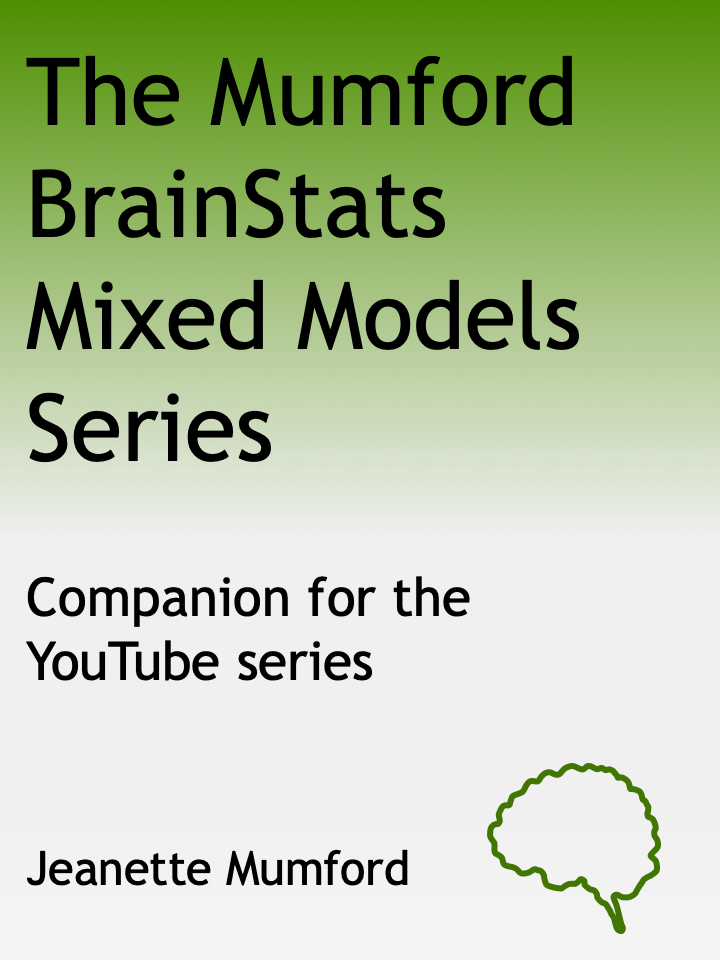
\includegraphics[width=250px]{./images/mixed_model_book_cover}

This is a collection of materials that accompanies a \href{https://www.youtube.com/watch?v=IGHm1XHFWMc\&list=PLB2iAtgpI4YEAUiEQ1ZnfMXY-yewNzn9z}{YouTube series on the MumfordBrainStats channel about mixed models}. Although I normall focus on material related to neuroimaging, this is for a general audience. Each of these chapters should be understandable without watching the video, but one would probably gain the most by watching the videos as well. The chapter titles indicate which video in the series goes along with that chapter. Not all videos have chapter (yet), since I'm only including chapters with code for now. In the future I may try to smooth this out more to read more like an actual book.

Although this series isn't necessarily set up to be a tutorial on how to run a mixed model properly, it would still be useful for somebody who is new to mixed models. I'm focusing on odds and ends that I've seen come up that I feel are less frequently discussed. Basically mistakes I've made or seen that I'd like to help you avoid. Interestingly, many of these mistakes are made by those with some knowledge of mixed models. I think they often arises from a ``knows enough to be dangerous'' situation. Do not misinterpret that as it is good to be dangerous, brave, make mistakes and then fix them. That's how we learn!

Specific goals of this series:

\begin{itemize}
\tightlist
\item
  Make it easier for you to conceptualize what a mixed model is doing
\item
  Describe the two stage random effects formulation and corresponding two stage summary statistics approach for modeling repeated measures data
\item
  Clarify when regularization is occurring and what it is doing
\item
  Clarifying what a conditional mode (BLUP) is and how they should \emph{not} be used
\item
  When a two stage summary statistics approach is likely okay to use
\end{itemize}

This series is still in development. Future topics will involve: crossed/nested random effects, tips for planning out your analysis setup, simplifying random effects structures (when is it okay) and hopefully some examples from the audience of this series about their trials and tribulations with mixed models. I'm also looking for solid ways to test model assumptions. So far I haven't found anything super satisfying.

For feedback, you can find me on twitter: @mumbrainstats.

\hypertarget{v3-simulation-using-2-stage-random-effects}{%
\chapter{V3: Simulation using 2-stage random effects}\label{v3-simulation-using-2-stage-random-effects}}

\hypertarget{relating-two-stage-random-effects-to-simulated-data-and-model-output}{%
\section{Relating two-stage random effects to simulated data and model output}\label{relating-two-stage-random-effects-to-simulated-data-and-model-output}}

\hypertarget{introduction-1}{%
\section{Introduction}\label{introduction-1}}

This chapter accompanies the 3rd video in the series, \href{https://youtu.be/OL6UezgpmPo}{``Simulating data using the 2-stage random effects formulation''}. The purpose of this chapter is to help in understanding the two-stage random effects formulation for mixed models by simulating data based on the formulation, analyzing the simulated data and comparing the two. This is a great way to wrap your head around what a mixed model is doing. This is written under the assumption that you have seen the first few videos in the \href{https://www.youtube.com/watch?v=IGHm1XHFWMc\&list=PLB2iAtgpI4YEAUiEQ1ZnfMXY-yewNzn9z}{Mixed Models series} on the MumfordBrainStats YouTube channel. If you haven't, go look for that playlist and watch those first. As discussed in the videos, this is not a perfect setup for the mixed models and not all mixed models can fit into this formulation, but it is a great way to understand mixed models. Sometimes it is helpful to see how repeated measures data are simulated in order to understand what the model is doing. In this case the values in the simulation will show up again when the data are fit using the lmer() function. Make sure to spend time matching up the values in the simulation code with the lmer output to increase your understanding of mixed models.

\hypertarget{data-simulation}{%
\section*{Data simulation}\label{data-simulation}}
\addcontentsline{toc}{section}{Data simulation}

The simulation follows the two-stage random effects formulation in reverse to make up some fake data that look similar to the Sleepstudy data. Typically simulations are used for estimating type I error and power, but they are great for learning too. The benefit in simulation is the truth is known and be compared with the estimates. Specifically,the true group intercept and slope as well as all of the variance parameters will be known in this case.

\hypertarget{review-of-the-two-stage-formulation}{%
\subsubsection*{Review of the two-stage formulation}\label{review-of-the-two-stage-formulation}}
\addcontentsline{toc}{subsubsection}{Review of the two-stage formulation}

Reviewing the two-stage formulation, recall the first stage of the model is \[Y_i = Z_i\beta_i + \epsilon_i, \: \epsilon_i\sim N(0, \sigma^2I_{n_i})\] and the second stage is \[\beta_i = A_i \beta + b_i, \: b_i \sim N(0,G).\] In these early examples \(A_i\) is an indentity matrix, so you can ignore it. This is because we're only averaging within-subject effects in these models. In this case \(Y_i\) contains the average reaction times for subject \(i\) over 10 days, \(Z_i\) is the design matrix with a column of 1s and a column for days (0-9), \(\beta_i\) is the vector with the slope and intercept for subject \(i\) and \(\sigma\) is the within-subject variance. Notably, this variance is assumed to be the same for all subjects, as it does not have an \(i\) subscript. Last, \(n_i\), the number of observations for subject \(i\), is assumed to be 10 for all subjects, so \(I_{n_i}\) is a \(n_i\times n_i\) identity matrix. Here's an example using the first subject in the data set (\(i\) would be 1),

\[\left[\begin{array}{c}
265 \\ 252 \\ 451 \\ 335 \\ 376 \\370 \\ 357 \\ 514 \\ 350 \\ 500 \end{array}\right] = \left[\begin{array}{cc}
1 & 0 \\
1 & 1 \\
1 & 2 \\
1 & 3 \\
1 & 4 \\
1 & 5 \\
1 & 6 \\
1& 7 \\
1 & 8 \\
1 & 9 \end{array}\right]\left[\begin{array}{c} \beta_{0, i} \\ \beta_{1, i}  \end{array}\right] + 
\left[\begin{array}{c}
\epsilon_1 \\
\epsilon_2 \\
\epsilon_3 \\
\epsilon_4 \\
\epsilon_5 \\
\epsilon_6 \\
\epsilon_7 \\
\epsilon_8 \\
\epsilon_9 \\
\epsilon_{10} 
\end{array}\right].\]

The second level is looks like: \[\left[\begin{array}{c}\beta_{0,i} \\ \beta_{1,i}\end{array}\right] =\left[\begin{array}{c}\beta_{0} \\ \beta_{1}\end{array}\right] + \left[\begin{array}{c}b_{0,i} \\ b_{1,i}\end{array}\right],\] since the interest is in the average intercept and slope across subjects.

\hypertarget{data-simulation-based-on-two-stage-formulation}{%
\subsubsection*{Data simulation based on two-stage formulation}\label{data-simulation-based-on-two-stage-formulation}}
\addcontentsline{toc}{subsubsection}{Data simulation based on two-stage formulation}

To simulate the data, one goes through the two stages backwards, starting with stage 2. This setting assumes the random slope and intercept are independent, the intercept's between-subject variance is \(24^2\) and slope's between-subject variance is \(10^2\), so \[G=\left[\begin{array}{cc} 24^2 & 0 \\ 0 & 10^2 \end{array}\right].\] Another way to think of this, since the slope and intercept are independent is: \(b_{0,i}\sim N(0, 24^2)\) and \(b_{1,i}\sim N(0, 10^2)\). The true group intercept and slope are assumed to be 251 and 10, respectively, so subject-specific slopes and intercepts are generated using the multivariate normal distribution
\[N\left(\left[\begin{array}{c} 251 \\ 10 \end{array}\right], \left[\begin{array}{cc} 24^2 & 0 \\ 0 & 10^2 \end{array}\right]\right).\]

It may not always be the case that the slope and intercept are independent. For example, sometimes the steepness of the slope may depend upon on where the subject started (the intercept). If they are very slow on the task on day 0, they may not decline as much over the following days compared to a person who starts off really fast. In this case, the off-diagonal of \(G\) would have a negative covariance value. In the interest of simplicity the independence assumption is used here, but the model fit will default to assuming they are correlated, which is fine. More on this to come.

To obtain the individual reaction times, the first stage is used based on the individual slope and intercept values that were generated with the multivariate Normal distribution above. Basically noise is added to that subject's true regression line, with a variance of \(30^2\) to yield the subject-specific reaction times. The simulated data are then complete and ready for analysis.

Read through the function and pay attention to where the betas, G and sigma are. Relate them to the equations above and later find their estimates in the lmer output! I've flagged the numbers to take note of with comments.

\begin{Shaded}
\begin{Highlighting}[]
\KeywordTok{library}\NormalTok{(ggplot2)}
\KeywordTok{library}\NormalTok{(lme4)}
\KeywordTok{library}\NormalTok{(lmerTest)}
\KeywordTok{library}\NormalTok{(MASS)}

\NormalTok{makeFakeSleepstudyData =}\StringTok{ }\ControlFlowTok{function}\NormalTok{(nsub)\{}
\NormalTok{  time =}\StringTok{ }\DecValTok{0}\OperatorTok{:}\DecValTok{9}
\NormalTok{  rt =}\StringTok{ }\KeywordTok{c}\NormalTok{() }\CommentTok{\# This will be filled in via the loop}
\NormalTok{  time.all =}\StringTok{ }\KeywordTok{rep}\NormalTok{(time, nsub)}
\NormalTok{  subid.all =}\StringTok{ }\KeywordTok{as.factor}\NormalTok{(}\KeywordTok{rep}\NormalTok{(}\DecValTok{1}\OperatorTok{:}\NormalTok{nsub, }\DataTypeTok{each =} \KeywordTok{length}\NormalTok{(time)))}
  
  \CommentTok{\# Step 1:  Generate the beta\_i\textquotesingle{}s.  }
\NormalTok{  G =}\StringTok{ }\KeywordTok{matrix}\NormalTok{(}\KeywordTok{c}\NormalTok{(}\DecValTok{24}\OperatorTok{\^{}}\DecValTok{2}\NormalTok{, }\DecValTok{0}\NormalTok{, }\DecValTok{0}\NormalTok{, }\DecValTok{10}\OperatorTok{\^{}}\DecValTok{2}\NormalTok{), }\DataTypeTok{nrow =} \DecValTok{2}\NormalTok{)   }\CommentTok{\#\#!!! <{-} REMEMBER THESE NUMBERS!!!!}
\NormalTok{  int.mean =}\StringTok{ }\DecValTok{251}  \CommentTok{\#\#!!! <{-} REMEMBER THESE NUMBERS TOO!!!!}
\NormalTok{  slope.mean =}\StringTok{ }\DecValTok{10}  \CommentTok{\#\#!!! <{-} REMEMBER THESE NUMBERS TOO!!!!}
\NormalTok{  sub.ints.slopes =}\StringTok{ }\KeywordTok{mvrnorm}\NormalTok{(nsub, }\KeywordTok{c}\NormalTok{(int.mean, slope.mean), G)}
\NormalTok{  sub.ints =}\StringTok{ }\NormalTok{sub.ints.slopes[,}\DecValTok{1}\NormalTok{]}
\NormalTok{  time.slopes =}\StringTok{ }\NormalTok{sub.ints.slopes[,}\DecValTok{2}\NormalTok{]}
  
  \CommentTok{\# Step 2:  Use the intercepts and slopes to generate RT data}
\NormalTok{  sigma =}\StringTok{ }\DecValTok{30}      \CommentTok{\#\#!!! <{-} THIS IS THE LAST NUMBER TO REMEMBER!!!! (sorry for yelling)}
  \ControlFlowTok{for}\NormalTok{ (i }\ControlFlowTok{in} \DecValTok{1}\OperatorTok{:}\NormalTok{nsub)\{}
\NormalTok{    rt.vec =}\StringTok{ }\NormalTok{sub.ints[i] }\OperatorTok{+}\StringTok{ }\NormalTok{time.slopes[i]}\OperatorTok{*}\NormalTok{time }\OperatorTok{+}\StringTok{ }\KeywordTok{rnorm}\NormalTok{(}\KeywordTok{length}\NormalTok{(time), }\DataTypeTok{sd =}\NormalTok{ sigma)}
\NormalTok{    rt =}\StringTok{ }\KeywordTok{c}\NormalTok{(rt, rt.vec)}
\NormalTok{  \}}
  
\NormalTok{  dat =}\StringTok{ }\KeywordTok{data.frame}\NormalTok{(rt, time.all, subid.all)}
  \KeywordTok{return}\NormalTok{(dat)}
\NormalTok{\}}
\end{Highlighting}
\end{Shaded}

\hypertarget{generate-and-plot-data}{%
\section{Generate and plot data}\label{generate-and-plot-data}}

The following generates data for 16 subjects and plots them. This should look somewhat like the real sleepstudy data that were discussed in an earlier video.

\begin{Shaded}
\begin{Highlighting}[]
\KeywordTok{set.seed}\NormalTok{(}\DecValTok{10}\NormalTok{) }\CommentTok{\# this ensures you get what I got here}
\NormalTok{dat =}\StringTok{ }\KeywordTok{makeFakeSleepstudyData}\NormalTok{(}\DecValTok{16}\NormalTok{)}
\KeywordTok{ggplot}\NormalTok{(}\DataTypeTok{data =}\NormalTok{ dat, }\KeywordTok{aes}\NormalTok{(}\DataTypeTok{x =}\NormalTok{ time.all, }\DataTypeTok{y =}\NormalTok{ rt)) }\OperatorTok{+}
\StringTok{  }\KeywordTok{geom\_line}\NormalTok{() }\OperatorTok{+}\StringTok{ }
\StringTok{  }\KeywordTok{geom\_point}\NormalTok{() }\OperatorTok{+}
\StringTok{  }\KeywordTok{facet\_wrap}\NormalTok{(}\OperatorTok{\textasciitilde{}}\NormalTok{subid.all)}
\end{Highlighting}
\end{Shaded}

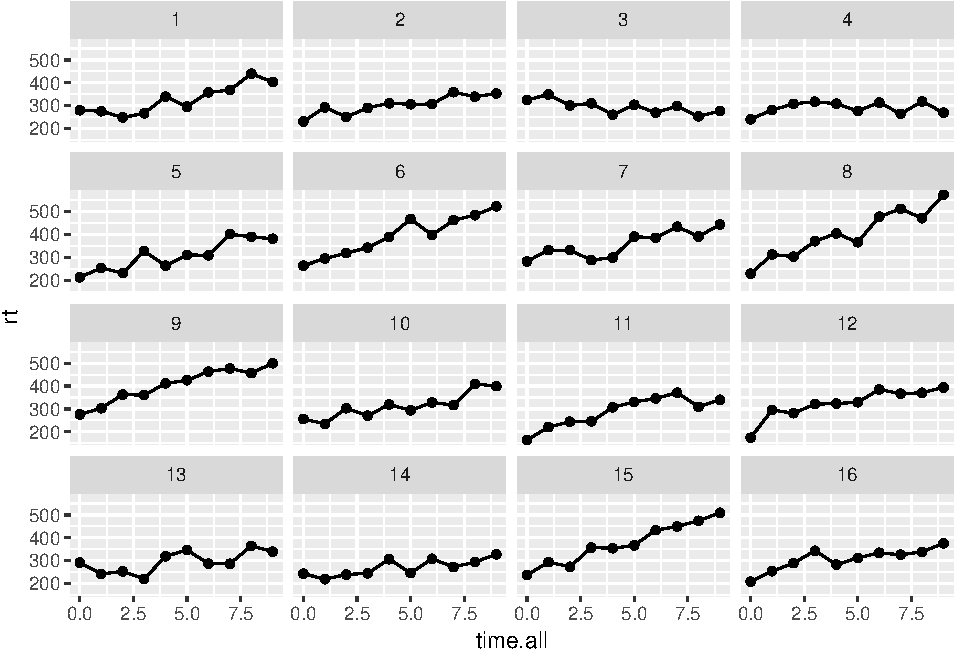
\includegraphics{1_video3_2_level_illustration_files/figure-latex/unnamed-chunk-2-1.pdf}

\hypertarget{run-model-and-compare-to-simulation-settings}{%
\section*{Run model and compare to simulation settings}\label{run-model-and-compare-to-simulation-settings}}
\addcontentsline{toc}{section}{Run model and compare to simulation settings}

Below is the appropriate model, which includes a random slope an intercept as well as a correlation between the two. To compare with the simulation values, first focus on the ``Random Effects'' section. This is where to find the between-subject variances for the slope and intercept as well as an estimate of the correlation between the two. The within-subject variance is also in this part of the output. Be generous when comparing these estimates with the truth since only 16 subjects with 10 observations each went into the analysis and the estimates are likely noisy. Recall from the \(G\) matrix above that the between subject variance for the intercept was set to \(24^2\), the between subject variance for the slope was \(10^2\) and the correlation between the two was 0. The variances roughly match the estimates, specifically 26.19\(^2\) and 9.77\(^2\). The correlation is estimated at -0.33. Later the topic of testing and simplifying random effects structures will be covered. Last, the within-subject variance was set to 30 in the simulations and is the Residual entry (last row) in the Random Effects section, 28.42\(^2\).

Moving on to the fixed effects column, our simulated intercept and slope values were 251 and 10, respectively. The estimates are pretty close: 253.56 and 16.59. Also take note of the degrees of freedom column. Why only 15? This actually makes a lot of sense when thinking about the two stage model. In the first stage a separate slope and intercept are estimated for each subject and then the second stage averages these. With 16 estimates, the degrees of freedom for an average would be 15, so this makes sense. Always report and ask others to report degrees of freedom, because it is a quick way to sense whether their random effects structure may have not been correct. More on this below.

\begin{Shaded}
\begin{Highlighting}[]
\KeywordTok{summary}\NormalTok{(}\KeywordTok{lmer}\NormalTok{(rt}\OperatorTok{\textasciitilde{}}\NormalTok{time.all }\OperatorTok{+}\StringTok{ }\NormalTok{(}\DecValTok{1}\OperatorTok{+}\NormalTok{time.all }\OperatorTok{|}\NormalTok{subid.all), dat))}
\end{Highlighting}
\end{Shaded}

\begin{verbatim}
## Linear mixed model fit by REML. t-tests use Satterthwaite's method [
## lmerModLmerTest]
## Formula: rt ~ time.all + (1 + time.all | subid.all)
##    Data: dat
## 
## REML criterion at convergence: 1588.5
## 
## Scaled residuals: 
##      Min       1Q   Median       3Q      Max 
## -2.43358 -0.64266  0.03094  0.72321  2.18928 
## 
## Random effects:
##  Groups    Name        Variance Std.Dev. Corr 
##  subid.all (Intercept) 685.73   26.186        
##            time.all     95.49    9.772   -0.33
##  Residual              807.84   28.423        
## Number of obs: 160, groups:  subid.all, 16
## 
## Fixed effects:
##             Estimate Std. Error      df t value Pr(>|t|)    
## (Intercept)  253.559      7.765  15.000  32.653 2.38e-15 ***
## time.all      16.594      2.565  15.000   6.469 1.06e-05 ***
## ---
## Signif. codes:  0 '***' 0.001 '**' 0.01 '*' 0.05 '.' 0.1 ' ' 1
## 
## Correlation of Fixed Effects:
##          (Intr)
## time.all -0.405
\end{verbatim}

\hypertarget{omitting-random-effects-can-inflate-type-i-error}{%
\section*{Omitting random effects can inflate Type I error}\label{omitting-random-effects-can-inflate-type-i-error}}
\addcontentsline{toc}{section}{Omitting random effects can inflate Type I error}

Omitting the random slope often a very bad idea. Generally, all within-subject variables that are continuous should be included as random effects unless there are convergence issues because there aren't enough data to estimate them. Definitely check out this paper by \href{https://www.sciencedirect.com/science/article/pii/S0749596X17300013}{Matusheck and others} as well as my \href{https://www.youtube.com/watch?v=pDNEgcl0YhI}{video} to learn about simplifying the random effects structure.
Below the random slope is omitted and the biggest impact is on the degrees of freedom, which are quite large now! Of course this results in a much smaller p-value. Generally there is a risk of inflated type I errors when omitting a random effect. It is best to start with a fully specified random effects structure and simplify if need be. This is why it is a good idea to report degrees of freedom and make sure they are reported when reviewing manuscripts.

\begin{Shaded}
\begin{Highlighting}[]
\NormalTok{bad.model =}\StringTok{ }\KeywordTok{lmer}\NormalTok{(rt}\OperatorTok{\textasciitilde{}}\NormalTok{time.all }\OperatorTok{+}\StringTok{ }\NormalTok{(}\DecValTok{1} \OperatorTok{|}\NormalTok{subid.all), dat)}
\KeywordTok{summary}\NormalTok{(bad.model)  }
\end{Highlighting}
\end{Shaded}

\begin{verbatim}
## Linear mixed model fit by REML. t-tests use Satterthwaite's method [
## lmerModLmerTest]
## Formula: rt ~ time.all + (1 | subid.all)
##    Data: dat
## 
## REML criterion at convergence: 1666.7
## 
## Scaled residuals: 
##      Min       1Q   Median       3Q      Max 
## -2.53803 -0.64128 -0.00096  0.67704  2.71143 
## 
## Random effects:
##  Groups    Name        Variance Std.Dev.
##  subid.all (Intercept) 1771     42.08   
##  Residual              1634     40.42   
## Number of obs: 160, groups:  subid.all, 16
## 
## Fixed effects:
##             Estimate Std. Error      df t value Pr(>|t|)    
## (Intercept)  253.559     12.082  21.768   20.99 6.23e-16 ***
## time.all      16.594      1.113 143.000   14.91  < 2e-16 ***
## ---
## Signif. codes:  0 '***' 0.001 '**' 0.01 '*' 0.05 '.' 0.1 ' ' 1
## 
## Correlation of Fixed Effects:
##          (Intr)
## time.all -0.414
\end{verbatim}

\hypertarget{summary}{%
\section*{Summary}\label{summary}}
\addcontentsline{toc}{section}{Summary}

The goal of this document was to shed some light on the two stage random effects structure to aid in understanding the output of lmer. In addition, the importance of including random effects was shown. Omitting random effects can greatly inflate the Type I error. If you have question about this document, do not hesitate to contact me via the MumfordBrainStats FB page or twitter.

\hypertarget{v4-introduction-to-regularization-in-mixed-models}{%
\chapter{V4: Introduction to regularization in mixed models}\label{v4-introduction-to-regularization-in-mixed-models}}

\hypertarget{what-is-this-regularization-and-why-dont-we-analyze-the-data-in-2-stages}{%
\section{What is this regularization and why don't we analyze the data in 2 stages?}\label{what-is-this-regularization-and-why-dont-we-analyze-the-data-in-2-stages}}

\hypertarget{introduction-2}{%
\section{Introduction}\label{introduction-2}}

This chapter is paired with the fourth video in the mixed model series, \href{https://youtu.be/sRhFeC-STdw}{What is this regularization and why don't we analyze the data in 2 stages?}. Although the two-stage formulation is a great way to conceptualize the mixed model, it also might inspire a shortcut for data analysis: the two-stage summary statistics approach. For those familiar with fMRI data, this is exactly what is done to analyze those data due to the complexity and structure of the data. The approaches vary greatly across software packages where the SPM approach is most similar to what will be done here, but I will not be making comparisons with or between fMRI software. There is a \href{https://www.ncbi.nlm.nih.gov/pubmed/19463958}{related paper}, written by myself and others that compares the models of different fMRI software packages.

There are many reasons why the all-in-one mixed model, which I will just call a mixed model or MM from now on, is better than using the two-stage summary statistics approach (called 2SSS from now on). For one, you are not allowed simplified or more complex random effects structures. For example, there may be cases where a within-subject variable will not be specified as random and you cannot really do this using 2SSS. There are other reasons that will come up as we work through this topic. The most compelling reason for the user might be that a mixed model takes about one line of code versus many lines of code for the summary statistics approach.

\hypertarget{regularization-key-difference}{%
\paragraph{Regularization: key difference}\label{regularization-key-difference}}

What about when the 2SSS and MM formulations are quite close? How does the mixed model result differ? Sometimes they'll be almost identical, but other times they will be quite different. Why? The short answer is the within-subject values related to the fixed effects are regularized in a mixed model and that is the focus here. This is a bit of a confusing statement because within-subject estimates are not actually estimated! Assume we are working with the sleepstudy data, which would include a within- and between-subject variability. Recall the mixed model equation, \[Y_i = X_i\beta + Z_ib_i + \epsilon_i,\] where \(Y_i\) is the dependent variable for subject \(i\), \(X_i\) is the design matrix for the fixed effects (see the last chapter for more details), \(\beta\) is the \emph{group} parameter vector, \(Z_i\) is a matrix for the random effects, \(b_i\) are the random effects describing between-subject variability, and \(\epsilon_i\) is describes the within-subject variability. There are not any within-subject parameters estimated in this model. The term, \(b_i\) is a random variable that describes the between-subject distribution, \(b_i \sim N(0, G)\). Importantly, the \(b_i\) are not estimated, but the corresponding covariance of the \(b_i\), \(G\), is estimated and serves as the between-subject variability estimate. Although the subject specific estimates are not estimated, the subjects with less data will contribute less to the estimate of the group parameter, \(\beta\). Much, much more exploration will be done on this topic as time goes on.

For now I would like to illustrate what the regularization looks like for means, but there isn't a perfect way to illustrate it. Typically the regularization is shown by comparing within-subject estimates to predicted within-subject estimates from the mixed model, based on values called BLUPS or best linear unbiased predictors. Some are not fans of this term, so I will simply refer to these as conditional modes, following the notation used by Douglas Bates, the author of the lme4 library. As stated in a draft of his book, ``it is an appealing acronym, I don't find the term particularly instructive (what is a `linear unbiased predictor' and in what context are these the `best'?) and prefer the term conditional mode.'' (book can be found \href{http://webcom.upmf-grenoble.fr/LIP/Perso/DMuller/M2R/R_et_Mixed/documents/Bates-book.pdf}{here} at the time of this writing). The reason why this isn't the perfect way of illustrating regularization is because it doesn't perfectly reflect how the regularization ends up impacting the group-level results. That will be the focus in the future, but now the goal is to understand that there is regularization happening.

The specific goal of the simulations below is to understand the impact of regularization by looking at estimates based on within-subject averages from the first stage of 2SSS and the conditional modes from mixed models. The first level estimates from 2SSS will be referred to as OLS (Ordinary Least Squares) estimates or \(\hat\beta_i^{OLS}\) and the conditional modes will be called just that or referred to as \(\hat\beta_i\).

\hypertarget{what-is-a-conditional-mode}{%
\paragraph{What is a conditional mode?}\label{what-is-a-conditional-mode}}

In an effort to keep equations at a minimum, I will explain conditional model conceptually. For more information I recommend looking at the Bates book I linked to above or the textbook, \href{https://www.amazon.com/Applied-Longitudinal-Analysis-Garrett-Fitzmaurice/dp/0470380276}{``Applied Longitudinal Analysis'' by Fitzmaurice, Laird and Ware}. To understand the difficulty of this problem, remind yourself that typically when we have a random variable that follows a distribution, say \(X \sim N(\mu, \sigma^2)\), we focus on the estimation of \(\mu\) and \(\sigma^2\). Asking what value \(X\) is doesn't even make much sense, since it is a a random variable. What can be done is to use the mode of the distribution as a prediction of \(X\), which is where the ``mode'' in ``conditional mode'' comes from. The conditioning part is somewhat simple. The mixed model equation above describes the distribution of \(Y_i\) but we want the distribution of \(b_i\) for a specific subject, \(i\). To get at this, the distribution of the random effects conditional on the \emph{data}, \(Y\), is used. The part of this process that is very different from when we estimate things, is that \emph{estimated} parameters (within-subject variance, between-subject covariance and fixed effects) are substituted in place of the truth in the distributions in order to derive these modes instead of the true values because they are unknown. This introduces an additional source of variability. The take-away is simply, again, the within-subject estimates are not estimated by default in a mixed model but we can predict them using conditional modes. These predictions can be quite noisy because they rely on estimates of parameters in order to specify the conditional distribution.

Next, some fake data will be generated and used to estimate some conditional modes and start building intuition about the regularization in mixed models. Fake data are used for the convenience of knowing the truth.

\hypertarget{simulated-data}{%
\section{Simulated data}\label{simulated-data}}

The simulated data consist of 10 subjects where 5 have 50 observations and 5 only have 5 observations from some type of behavioral experiment measuring reaction time. As in the last chapter, the two-stage random effects formulation will be used to simulate the data.

\begin{Shaded}
\begin{Highlighting}[]
\KeywordTok{library}\NormalTok{(lme4)}
\KeywordTok{library}\NormalTok{(lmerTest)}
\KeywordTok{library}\NormalTok{(ggplot2)}
\CommentTok{\# Simulate true subject{-}specific means:}
\NormalTok{nsub =}\StringTok{ }\DecValTok{10}
\NormalTok{btwn.sub.sd =}\StringTok{ }\DecValTok{10}
\CommentTok{\#within{-}subject means }
\NormalTok{win.means =}\StringTok{ }\KeywordTok{rnorm}\NormalTok{(nsub, }\DataTypeTok{mean =} \DecValTok{250}\NormalTok{, }\DataTypeTok{sd =}\NormalTok{ btwn.sub.sd)}

\CommentTok{\# Simualte data for each subject by wiggling around their means}
\NormalTok{win.sub.sd =}\StringTok{ }\DecValTok{20}
\CommentTok{\# The following indicates how many data per subject, the first 5 only have 5 observations.}
\NormalTok{n.per.sub =}\StringTok{ }\KeywordTok{rep}\NormalTok{(}\DecValTok{50}\NormalTok{, nsub)}
\NormalTok{n.per.sub[}\DecValTok{1}\OperatorTok{:}\DecValTok{5}\NormalTok{] =}\StringTok{ }\DecValTok{5}
\NormalTok{rt =}\StringTok{ }\KeywordTok{c}\NormalTok{()}
\NormalTok{subid =}\StringTok{ }\KeywordTok{c}\NormalTok{()}
\ControlFlowTok{for}\NormalTok{ (i }\ControlFlowTok{in} \DecValTok{1}\OperatorTok{:}\NormalTok{nsub)\{}
\NormalTok{  rt.loop =}\StringTok{ }\KeywordTok{rnorm}\NormalTok{(n.per.sub[i], win.means[i], }\DataTypeTok{sd =}\NormalTok{ win.sub.sd)}
\NormalTok{  rt =}\StringTok{ }\KeywordTok{c}\NormalTok{(rt, rt.loop)}
\NormalTok{  subid =}\StringTok{ }\KeywordTok{c}\NormalTok{(subid, }\KeywordTok{rep}\NormalTok{(i, n.per.sub[i]))}
\NormalTok{\}}
\NormalTok{dat =}\StringTok{ }\KeywordTok{data.frame}\NormalTok{(subid, rt)}
\end{Highlighting}
\end{Shaded}

Here is a plot of the resulting data. As you can see the first five subjects have much less data than the rest of the subjects. This was done on purpose to illustrate the regularization since the factor that impacts the regularization is the amount of data within-subject. There is much more to this, but it will be covered in the following chapters.

\begin{Shaded}
\begin{Highlighting}[]
\KeywordTok{ggplot}\NormalTok{(dat, }\KeywordTok{aes}\NormalTok{(}\DataTypeTok{x=}\KeywordTok{as.factor}\NormalTok{(subid), }\DataTypeTok{y =}\NormalTok{ rt)) }\OperatorTok{+}
\StringTok{  }\KeywordTok{geom\_boxplot}\NormalTok{() }\OperatorTok{+}\StringTok{ }
\StringTok{  }\KeywordTok{geom\_jitter}\NormalTok{(}\DataTypeTok{shape=}\DecValTok{16}\NormalTok{, }\DataTypeTok{position=}\KeywordTok{position\_jitter}\NormalTok{(}\FloatTok{0.2}\NormalTok{)) }\OperatorTok{+}
\StringTok{  }\KeywordTok{xlab}\NormalTok{(}\StringTok{"Subject"}\NormalTok{)}\OperatorTok{+}\KeywordTok{ylab}\NormalTok{(}\StringTok{"RT"}\NormalTok{)}
\end{Highlighting}
\end{Shaded}

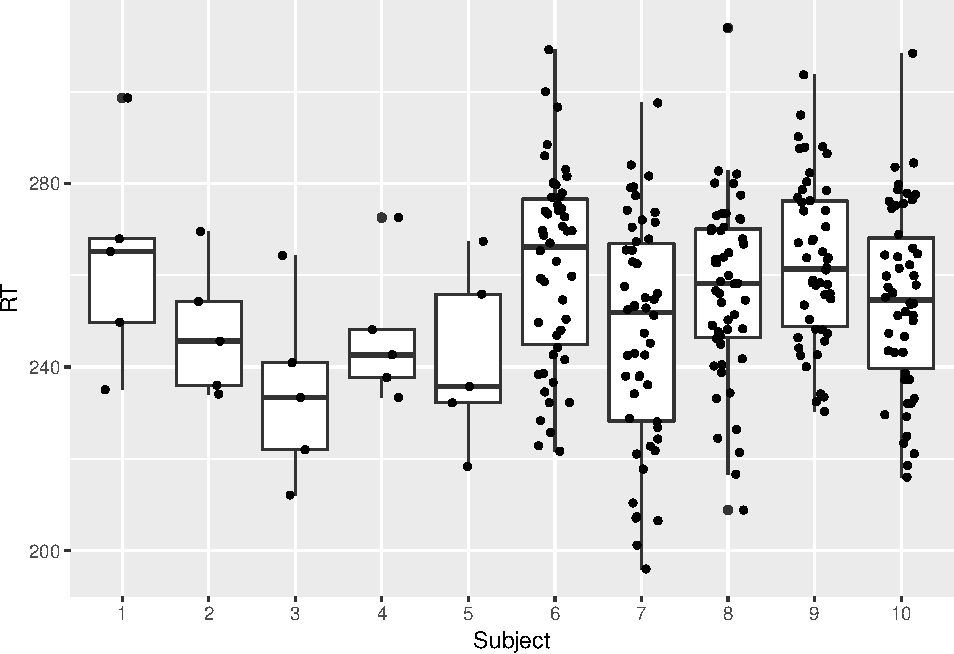
\includegraphics{2_video4_two_stage_temptation_files/figure-latex/unnamed-chunk-3-1.pdf}

\hypertarget{stage-summary-statistics-approach-compared-to-conditional-modes}{%
\section{2-stage summary statistics approach compared to conditional modes}\label{stage-summary-statistics-approach-compared-to-conditional-modes}}

Now that the data have been generated, the 2SSS uses a within-subject OLS linear regression model to obtain the within-subject means, \(\hat\beta_i^{OLS}\) and then these are averaged in a second OLS model to obtain the group estimates. The following runs these two stages and also estimates the proper mixed model.

\begin{Shaded}
\begin{Highlighting}[]
\CommentTok{\# Stage 1}
\NormalTok{stage1.est =}\StringTok{ }\KeywordTok{rep}\NormalTok{(}\OtherTok{NA}\NormalTok{, nsub)}
\ControlFlowTok{for}\NormalTok{ (i }\ControlFlowTok{in} \DecValTok{1}\OperatorTok{:}\NormalTok{nsub)\{}
  \CommentTok{\# Estimating the mean RT via OLS}
\NormalTok{  mod.loop =}\StringTok{ }\KeywordTok{lm}\NormalTok{(rt }\OperatorTok{\textasciitilde{}}\StringTok{ }\DecValTok{1}\NormalTok{, dat[dat}\OperatorTok{$}\NormalTok{subid}\OperatorTok{==}\NormalTok{i,])}
\NormalTok{  stage1.est[i] =}\StringTok{ }\NormalTok{mod.loop}\OperatorTok{$}\NormalTok{coef[}\DecValTok{1}\NormalTok{]}
\NormalTok{\}}

\CommentTok{\#Stage 2}
\KeywordTok{summary}\NormalTok{(}\KeywordTok{lm}\NormalTok{(stage1.est }\OperatorTok{\textasciitilde{}}\StringTok{ }\DecValTok{1}\NormalTok{))}
\end{Highlighting}
\end{Shaded}

\begin{verbatim}
## 
## Call:
## lm(formula = stage1.est ~ 1)
## 
## Residuals:
##      Min       1Q   Median       3Q      Max 
## -17.1940  -4.7550  -0.5041   8.5768  11.5654 
## 
## Coefficients:
##             Estimate Std. Error t value Pr(>|t|)    
## (Intercept)  251.754      3.047   82.62 2.82e-14 ***
## ---
## Signif. codes:  0 '***' 0.001 '**' 0.01 '*' 0.05 '.' 0.1 ' ' 1
## 
## Residual standard error: 9.636 on 9 degrees of freedom
\end{verbatim}

\begin{Shaded}
\begin{Highlighting}[]
\CommentTok{\#\# Proper mixed model}
\NormalTok{mod.lmer =}\StringTok{ }\KeywordTok{lmer}\NormalTok{(rt }\OperatorTok{\textasciitilde{}}\StringTok{ }\DecValTok{1} \OperatorTok{+}\StringTok{ }\NormalTok{(}\DecValTok{1}\OperatorTok{|}\NormalTok{subid), dat)}
\KeywordTok{summary}\NormalTok{(mod.lmer)}
\end{Highlighting}
\end{Shaded}

\begin{verbatim}
## Linear mixed model fit by REML. t-tests use Satterthwaite's method [
## lmerModLmerTest]
## Formula: rt ~ 1 + (1 | subid)
##    Data: dat
## 
## REML criterion at convergence: 2449.6
## 
## Scaled residuals: 
##      Min       1Q   Median       3Q      Max 
## -2.54753 -0.69671  0.02651  0.72996  2.80661 
## 
## Random effects:
##  Groups   Name        Variance Std.Dev.
##  subid    (Intercept)  39.81    6.309  
##  Residual             423.42   20.577  
## Number of obs: 275, groups:  subid, 10
## 
## Fixed effects:
##             Estimate Std. Error      df t value Pr(>|t|)    
## (Intercept)  253.885      2.638   6.206   96.25 4.35e-11 ***
## ---
## Signif. codes:  0 '***' 0.001 '**' 0.01 '*' 0.05 '.' 0.1 ' ' 1
\end{verbatim}

Comparing the lm summary to the fixed effects summary from the lmer model, the results are almost identical. Although this makes it tempting for many to use 2SSS instead of a mixed model, the next series of videos will set these two modeling approaches apart.

For practice, find the within- and between-subject variance estimates in the lmer summary and compare to the true values used in the simulation.

\hypertarget{ols-versus-conditional-modes}{%
\section{OLS versus conditional modes}\label{ols-versus-conditional-modes}}

To see the impact of regularization it is necessary to predict the subject-specific values from lmer. As mentioned above, these values are not estimated in any way shape or form during the modeling process above. In the following, the code asks lmer for these predicted values.

\begin{Shaded}
\begin{Highlighting}[]
\CommentTok{\# Mixed model conditional modes}
\NormalTok{mmcm =}\StringTok{ }\KeywordTok{coef}\NormalTok{(mod.lmer)}\OperatorTok{$}\NormalTok{subid[, }\DecValTok{1}\NormalTok{]}
\end{Highlighting}
\end{Shaded}

The following plot compares the mixed model estimates based on the conditional mean (MMCM, orange) in orange to the within-subject OLS estimates (OLS, blue) from the first stage of the 2SSS. The true mean was\ldots.well, the reader should practice understanding the above code by finding that themselves. Once you've located that value above, you will notice that the orange dots (MMCM) are shrunken toward the overall group mean compared to the blue OLS estimates. That is a result of the regularization. Recall the first 5 subjects had much less data than the last 5 subjects, which means there's more likely to be \emph{more} regularization for the first 5 subjects. I will introduce an equation that describes this exactly in the next chapter, but for now just note the basic trend. It is easiest to see if comparing subject 1 to subject 9. In both cases their within-subject OLS estimates are almost identical, but the MMCM estimate for subject 1 is much smaller! This is reflecting the fact that subject 1 had much less data than subject 9.

\begin{Shaded}
\begin{Highlighting}[]
\NormalTok{subject =}\StringTok{ }\KeywordTok{rep}\NormalTok{(}\KeywordTok{c}\NormalTok{(}\DecValTok{1}\OperatorTok{:}\NormalTok{nsub), }\DecValTok{2}\NormalTok{)}
\NormalTok{estimate =}\StringTok{ }\KeywordTok{c}\NormalTok{(mmcm, stage1.est)}
\NormalTok{estimate.type =}\StringTok{ }\KeywordTok{rep}\NormalTok{(}\KeywordTok{c}\NormalTok{(}\StringTok{"MMCM"}\NormalTok{, }\StringTok{"OLS"}\NormalTok{), }\DataTypeTok{each =}\NormalTok{ nsub)}
\NormalTok{dat.sub.est =}\StringTok{ }\KeywordTok{data.frame}\NormalTok{(subject, estimate, estimate.type)}

\CommentTok{\# Nice colorblind{-}friendly pallette}
\CommentTok{\# http://www.cookbook{-}r.com/Graphs/Colors\_(ggplot2)/\#a{-}colorblind{-}friendly{-}palette}
\NormalTok{cbPalette <{-}}\StringTok{ }\KeywordTok{c}\NormalTok{(}\StringTok{"\#E69F00"}\NormalTok{, }\StringTok{"\#56B4E9"}\NormalTok{, }\StringTok{"\#009E73"}\NormalTok{, }\StringTok{"\#F0E442"}\NormalTok{, }\StringTok{"\#0072B2"}\NormalTok{, }\StringTok{"\#D55E00"}\NormalTok{, }\StringTok{"\#CC79A7"}\NormalTok{,}\StringTok{"\#999999"}\NormalTok{)}


\KeywordTok{ggplot}\NormalTok{(dat.sub.est, }\KeywordTok{aes}\NormalTok{(}\DataTypeTok{x =}\NormalTok{ subject, }\DataTypeTok{y =}\NormalTok{ estimate, }
                        \DataTypeTok{color =}\NormalTok{ estimate.type)) }\OperatorTok{+}
\StringTok{  }\KeywordTok{geom\_point}\NormalTok{()}\OperatorTok{+}\StringTok{ }\KeywordTok{scale\_colour\_manual}\NormalTok{(}\DataTypeTok{values=}\NormalTok{cbPalette) }\OperatorTok{+}\StringTok{ }\KeywordTok{xlab}\NormalTok{(}\StringTok{"Subject"}\NormalTok{)}\OperatorTok{+}\KeywordTok{ylab}\NormalTok{(}\StringTok{"RT"}\NormalTok{) }\OperatorTok{+}\StringTok{ }\KeywordTok{labs}\NormalTok{(}\DataTypeTok{color =} \StringTok{"Estimate Type"}\NormalTok{) }\OperatorTok{+}\StringTok{ }
\StringTok{  }\KeywordTok{scale\_x\_continuous}\NormalTok{(}\DataTypeTok{breaks =} \KeywordTok{seq}\NormalTok{(}\DecValTok{0}\NormalTok{ , }\DecValTok{10}\NormalTok{, }\DecValTok{1}\NormalTok{), }\DataTypeTok{minor\_breaks=}\KeywordTok{seq}\NormalTok{(}\DecValTok{0}\NormalTok{, }\DecValTok{10}\NormalTok{,}\DecValTok{1}\NormalTok{))}
\end{Highlighting}
\end{Shaded}

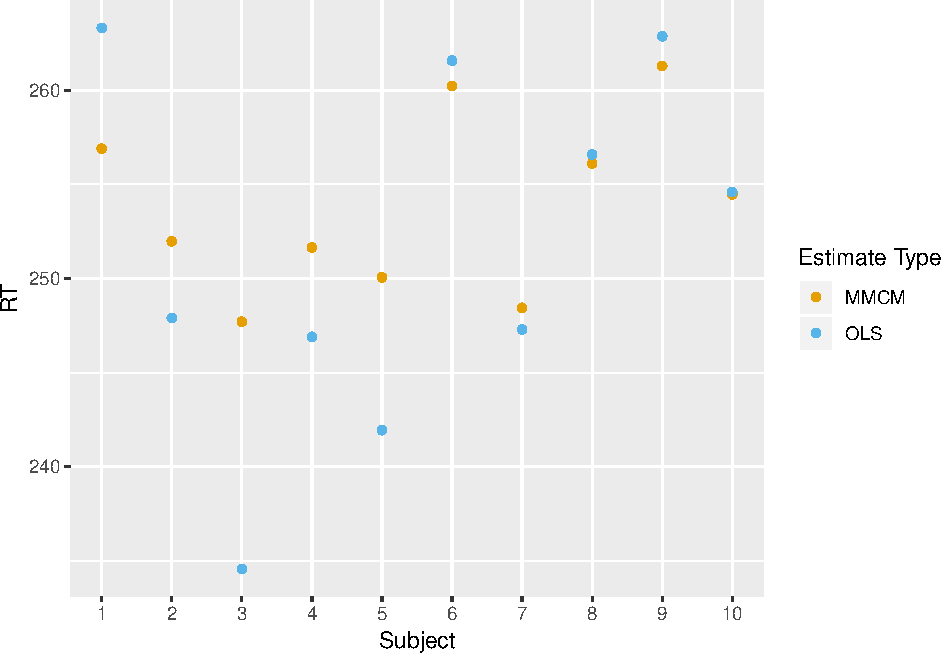
\includegraphics{2_video4_two_stage_temptation_files/figure-latex/unnamed-chunk-6-1.pdf}

\hypertarget{summary-1}{%
\section{Summary}\label{summary-1}}

This document is just a taste of what is to come. This is just a beginning to convince folks analyzing data that data analysis can be done better without using the two-stage summary statistics model, so don't be tempted! There are cases where you will not have a choice, but generally you will be better off with a mixed model. Future chapters will help clarify when these two approaches will yield similar results.

Although not a perfect way to view the phenomenon, conditional mode-based within-subject estimates from mixed models help in understanding the regularization that happens in the mixed model framework. On the surface it can be thought of as trying to stabilize the estimate from subjects with less data. The important take away for now is that this is driven by the amount of data within-subject.

What inspired this series is that when I explained this point to my colleague she immediately wanted to know how this regularization might impact her between-subject analyses. For example, what if in the fake data above the first 5 subjects were patients and the last 5 were controls. It is a reasonable scenario that some patients may have less data than controls, which is definitely the case for my colleague's data. If the patients' estimates are shrunken toward the overall mean because they have less data, could that introduce false positives or reduce power? A really great question! That is what the focus will be in the following chapters where I will use simulated data to compared different modeling approaches. It will also reveal the misleading nature of these conditional mode estimates.

\hypertarget{v5-conditional-modes-vs-means}{%
\chapter{V5: Conditional modes vs means}\label{v5-conditional-modes-vs-means}}

\hypertarget{relationship-between-mixed-model-conditional-modes-aka-blups-and-ols-estimates}{%
\section{Relationship between mixed model conditional modes (aka BLUPS) and OLS estimates}\label{relationship-between-mixed-model-conditional-modes-aka-blups-and-ols-estimates}}

\hypertarget{introduction-3}{%
\section{Introduction}\label{introduction-3}}

This chapter accompanies the fifth video in the mixed models series, \href{https://youtu.be/QqEUKlKPos4}{``Relationship between mixed model conditional modes (aka BLUPS) and OLS estimates''}.
In the last chapter, mixed models were contrasted to using the two-stage summary statistics model (2SSS) focusing on the regularization that is built into mixed models. Specifically, the ordinary least squares (OLS) estimates from stage 1 of 2SSS were compared to the conditional mode-based subject predictions from mixed models to show the regularization of the estimates, within-subject, in the mixed model setting. Although the conditional mode predictions are not perfect, that exploration will be started in the next segment. Here the focus is on the details of the relationship of the OLS estimates and the conditional mode estimates as there is an equation that describes this relationship! Why is this exciting? Because it helps build intuition about when these two approaches will greatly differ. I will be briefly discussing this equation below, but for more technical details see section 8.7 of the \href{https://www.amazon.com/Applied-Longitudinal-Analysis-Garrett-Fitzmaurice/dp/0470380276}{Applied Longitudinal Analysis text by Fitzmaurice and others}.

I will stick with the simplified example from last time, where there are multiple measures of reaction time for each subject and the interest is in the mean. Here's a reminder of how the data were generated (exactly the same code as last time and seed is fixed so same numbers are generated):

\begin{Shaded}
\begin{Highlighting}[]
\KeywordTok{library}\NormalTok{(lme4)}
\KeywordTok{library}\NormalTok{(lmerTest)}
\KeywordTok{library}\NormalTok{(ggplot2)}
\KeywordTok{set.seed}\NormalTok{(}\DecValTok{1850}\NormalTok{)  }\CommentTok{\# This is simply fixing the seed so the code always gives the same result.  }
\CommentTok{\#Obviously omit this if you are running new simulations}

\CommentTok{\# Simulate true subject{-}specific means:}
\NormalTok{nsub =}\StringTok{ }\DecValTok{10}
\NormalTok{btwn.sub.sd =}\StringTok{ }\DecValTok{10}
\CommentTok{\#within{-}subject means}
\NormalTok{win.means =}\StringTok{ }\KeywordTok{rnorm}\NormalTok{(nsub, }\DataTypeTok{mean =} \DecValTok{250}\NormalTok{, }\DataTypeTok{sd =}\NormalTok{ btwn.sub.sd)}

\CommentTok{\# Simualte data for each subject by wiggling around their means}
\NormalTok{win.sub.sd =}\StringTok{ }\DecValTok{20}
\CommentTok{\# The following indicates how many data per subject, the first 5 only have 5 observations.}
\NormalTok{n.per.sub =}\StringTok{ }\KeywordTok{rep}\NormalTok{(}\DecValTok{50}\NormalTok{, nsub)}
\NormalTok{n.per.sub[}\DecValTok{1}\OperatorTok{:}\DecValTok{5}\NormalTok{] =}\StringTok{ }\DecValTok{5}
\NormalTok{rt =}\StringTok{ }\KeywordTok{c}\NormalTok{()}
\NormalTok{subid =}\StringTok{ }\KeywordTok{c}\NormalTok{()}
\ControlFlowTok{for}\NormalTok{ (i }\ControlFlowTok{in} \DecValTok{1}\OperatorTok{:}\NormalTok{nsub)\{}
\NormalTok{  rt.loop =}\StringTok{ }\KeywordTok{rnorm}\NormalTok{(n.per.sub[i], win.means[i], }\DataTypeTok{sd =}\NormalTok{ win.sub.sd)}
\NormalTok{  rt =}\StringTok{ }\KeywordTok{c}\NormalTok{(rt, rt.loop)}
\NormalTok{  subid =}\StringTok{ }\KeywordTok{c}\NormalTok{(subid, }\KeywordTok{rep}\NormalTok{(i, n.per.sub[i]))}
\NormalTok{\}}
\NormalTok{dat =}\StringTok{ }\KeywordTok{data.frame}\NormalTok{(subid, rt)}
\end{Highlighting}
\end{Shaded}

\hypertarget{the-equation-for-shrinkage}{%
\section{The equation for shrinkage}\label{the-equation-for-shrinkage}}

As a reminder, the formula for the mixed model is: \[Y_i = X_i\beta + A_ib_i + \epsilon_i. \] With the data setup for this chapter, \(Y_i\) is a vector of reaction times for subject \(i\), \(X_i = Z_iA_i\) simplifies to \(Z_i\), since we are only estimating an average over subjects. Since we are also only estimating a within-subject average, \(Z_i\) is simply a column of 1s with length \(N_i\), the number of observations for subject \(i\). The random effect, \(b_i\), is of length 1 since only a random intercept in necessary. Specifically, \(b_i\sim N(0, G)\), where \(G\) is a scalar, and \(\epsilon_i\) describes the within-subject variability, \(\epsilon_i \sim N(0, \sigma^2I_{N_i})\). If needed, review the more detailed explanation of these matrices and vectors from previous lessons.

The following are what we need to focus on and I quickly relate the parameters to the output of the code below, which is repeated code from the last lesson.

\begin{itemize}
\tightlist
\item
  \(\hat\beta\): The fixed effects (group) estimate of the mean from the mixed model. This is the estimated group intercept, 253.88 below.
\item
  \(\hat\beta_i\): The conditional mode, predicted value for subject \(i\) from the mixed model. These values are stored in the mmcm vector created with the coef function below.
\item
  \(\hat\beta_i^{OLS}\): The OLS-based estimate from stage 1 of 2SSS, \(Y_i = Z_i\beta_i^{OLS} + \gamma_i.\) These are stored in the stage1.est vector below.
\item
  \(N_i\): the number of data points for subject \(i\). For now this is 5 for the first 5 subjects and 50 for the second 5 subjects.
\item
  \(G\) and \(\sigma^2\): Between-subject variance/covariance matrix and within-subject variance. In this case we'll work with the estimates which are \(G=6.309^2\) and \(\sigma^2 = 20.577^2\) and stored in vcov.vals. Find them in the mixed model output below.
\end{itemize}

\begin{Shaded}
\begin{Highlighting}[]
\CommentTok{\# Stage 1}
\NormalTok{stage1.est =}\StringTok{ }\KeywordTok{rep}\NormalTok{(}\OtherTok{NA}\NormalTok{, nsub)}
\ControlFlowTok{for}\NormalTok{ (i }\ControlFlowTok{in} \DecValTok{1}\OperatorTok{:}\NormalTok{nsub)\{}
  \CommentTok{\# Estimating the mean RT via linear regression}
\NormalTok{  mod.loop =}\StringTok{ }\KeywordTok{lm}\NormalTok{(rt }\OperatorTok{\textasciitilde{}}\StringTok{ }\DecValTok{1}\NormalTok{, dat[dat}\OperatorTok{$}\NormalTok{subid}\OperatorTok{==}\NormalTok{i,])}
\NormalTok{  stage1.est[i] =}\StringTok{ }\NormalTok{mod.loop}\OperatorTok{$}\NormalTok{coef[}\DecValTok{1}\NormalTok{]}
\NormalTok{\}}
\NormalTok{mod.lmer =}\StringTok{ }\KeywordTok{lmer}\NormalTok{(rt }\OperatorTok{\textasciitilde{}}\StringTok{ }\DecValTok{1} \OperatorTok{+}\StringTok{ }\NormalTok{(}\DecValTok{1}\OperatorTok{|}\NormalTok{subid), dat)}
\KeywordTok{summary}\NormalTok{(mod.lmer)}
\end{Highlighting}
\end{Shaded}

\begin{verbatim}
## Linear mixed model fit by REML. t-tests use Satterthwaite's method [
## lmerModLmerTest]
## Formula: rt ~ 1 + (1 | subid)
##    Data: dat
## 
## REML criterion at convergence: 2449.6
## 
## Scaled residuals: 
##      Min       1Q   Median       3Q      Max 
## -2.54753 -0.69671  0.02651  0.72996  2.80661 
## 
## Random effects:
##  Groups   Name        Variance Std.Dev.
##  subid    (Intercept)  39.81    6.309  
##  Residual             423.42   20.577  
## Number of obs: 275, groups:  subid, 10
## 
## Fixed effects:
##             Estimate Std. Error      df t value Pr(>|t|)    
## (Intercept)  253.885      2.638   6.206   96.25 4.35e-11 ***
## ---
## Signif. codes:  0 '***' 0.001 '**' 0.01 '*' 0.05 '.' 0.1 ' ' 1
\end{verbatim}

\begin{Shaded}
\begin{Highlighting}[]
\NormalTok{mmcm =}\StringTok{ }\KeywordTok{coef}\NormalTok{(mod.lmer)}\OperatorTok{$}\NormalTok{subid[, }\DecValTok{1}\NormalTok{]}
\NormalTok{vcov.vals =}\StringTok{ }\KeywordTok{as.data.frame}\NormalTok{(}\KeywordTok{VarCorr}\NormalTok{(mod.lmer)) }\CommentTok{\#random effects values}
\NormalTok{beta.hat =}\StringTok{ }\KeywordTok{summary}\NormalTok{(mod.lmer)}\OperatorTok{$}\NormalTok{coefficients[}\DecValTok{1}\NormalTok{]}
\end{Highlighting}
\end{Shaded}

If one is interested in the derivation of the relationship between \(\hat\beta_i\) and \(\hat\beta_i^{OLS}\), see section 8.7 of the \href{https://www.amazon.com/Applied-Longitudinal-Analysis-Garrett-Fitzmaurice/dp/0470380276}{Applied Longitudinal Analysis text by Fitzmaurice and others}. The end result is: \[\hat\beta_i = W_i\hat\beta_i^{OLS}+(I_q-W_i)A_i\hat\beta,\]
where \(q\) is the dimension of G and \[W_i= G\{G+\sigma^2(Z_i'Z_i)^{-1}\}^{-1}.\]
Before tackling what \(W_i\) is, exactly, focus on the general structure of the relationship assuming \(A_i\) is the identity matrix (more on this in a future lesson). If the weight, \(W_i\), is very small, then what counts the most toward the estimate of \(\hat\beta_i\) is the fixed effects estimate of \(\beta\). From the last lesson you might suspect that \(W_i\) will be small when a subject has less data, since that's when more regularization was present. On the other hand, if \(W_i\) is very large, the conditional mode-based estimate from the mixed model will look very similar to the within-subject estimate from the first stage of 2SSS, which is what we saw for the subjects who had more data in the last lesson.

Let's test that theory by deriving \(W_i\) for our specific model. Recall \(Z_i\) is just a column of 1s of length \(N_i\), so \((Z_i'Z_i)^{-1} = 1/N_i\) and \(G\) is just a scalar (between-subject variance of the mean), so we have: \[W_i  = \frac{G}{G+\sigma^2/N_i}=\frac{6.31^2}{6.31^2+20.58^2/N_i}.\]

Now it is crystal clear that our suspicions from the last lesson are true: for small \(N_i\) the overall weight will be small, favoring \(\hat\beta\) and if \(N_i\) is large, the overall weight will be large, favoring \(\hat\beta^{OLS}_i\). Here's a plot of the weight as a function of \(N_i\)

\begin{Shaded}
\begin{Highlighting}[]
\NormalTok{Ni.plot =}\StringTok{ }\DecValTok{1}\OperatorTok{:}\DecValTok{50}
\NormalTok{Wi.plot =}\StringTok{ }\NormalTok{vcov.vals[}\DecValTok{1}\NormalTok{,}\DecValTok{4}\NormalTok{]}\OperatorTok{/}\NormalTok{(vcov.vals[}\DecValTok{1}\NormalTok{,}\DecValTok{4}\NormalTok{] }\OperatorTok{+}\StringTok{ }\NormalTok{vcov.vals[}\DecValTok{2}\NormalTok{,}\DecValTok{4}\NormalTok{]}\OperatorTok{/}\NormalTok{Ni.plot)}
\NormalTok{datplot =}\StringTok{ }\KeywordTok{data.frame}\NormalTok{(Ni.plot, Wi.plot)}
\KeywordTok{ggplot}\NormalTok{(datplot, }\KeywordTok{aes}\NormalTok{(}\DataTypeTok{x=}\NormalTok{Ni.plot, }\DataTypeTok{y =}\NormalTok{Wi.plot)) }\OperatorTok{+}\StringTok{ }\KeywordTok{geom\_point}\NormalTok{() }\OperatorTok{+}\KeywordTok{labs}\NormalTok{(}\DataTypeTok{y=}\KeywordTok{expression}\NormalTok{(W[i]), }\DataTypeTok{x =} \KeywordTok{expression}\NormalTok{(N[i]))}
\end{Highlighting}
\end{Shaded}

\begin{center}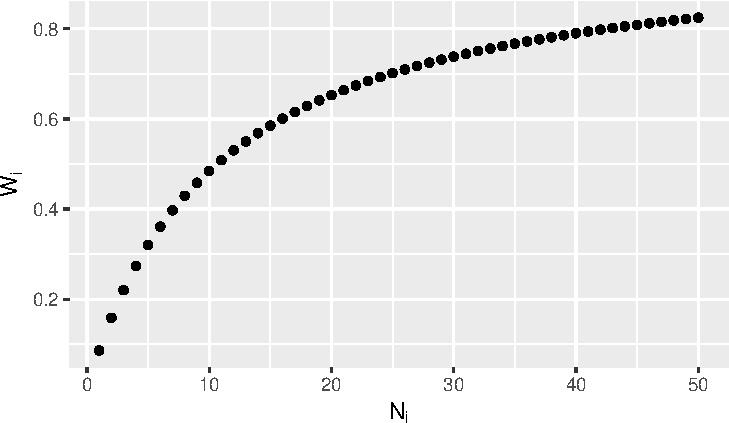
\includegraphics{3_video5_win_sub_mns_vs_cond_modes_files/figure-latex/unnamed-chunk-4-1} \end{center}

Granted things will be more difficult if the model has a slope and an intercept (when G is a matrix) and when between-subject variables are included (\(A_i\) will not be the identity), but we will deal with that later.

\hypertarget{verifying-coef.lmer-is-following-the-equation}{%
\section{Verifying coef.lmer is following the equation}\label{verifying-coef.lmer-is-following-the-equation}}

Although it is satisfying to find this equation it is only fully satisfying if that is what lmer is doing when we ask for the conditional modes. The following verifies this for each subject.

\begin{Shaded}
\begin{Highlighting}[]
\NormalTok{Wi =}\StringTok{ }\NormalTok{vcov.vals[}\DecValTok{1}\NormalTok{,}\DecValTok{4}\NormalTok{]}\OperatorTok{/}\NormalTok{(vcov.vals[}\DecValTok{1}\NormalTok{,}\DecValTok{4}\NormalTok{] }\OperatorTok{+}\StringTok{ }\NormalTok{vcov.vals[}\DecValTok{2}\NormalTok{,}\DecValTok{4}\NormalTok{]}\OperatorTok{/}\NormalTok{n.per.sub) }
\CommentTok{\# See first code chunk for n.per.sub}
\NormalTok{cond.mode.est =}\StringTok{ }\NormalTok{Wi}\OperatorTok{*}\NormalTok{stage1.est }\OperatorTok{+}\StringTok{ }\NormalTok{(}\DecValTok{1}\OperatorTok{{-}}\NormalTok{Wi)}\OperatorTok{*}\NormalTok{beta.hat}

\CommentTok{\# Stack my estimates on top of lmer\textquotesingle{}s conditional model estimates}
\KeywordTok{rbind}\NormalTok{(cond.mode.est, mmcm)                     }
\end{Highlighting}
\end{Shaded}

\begin{verbatim}
##                   [,1]     [,2]     [,3]    [,4]     [,5]     [,6]     [,7]
## cond.mode.est 256.9017 251.9737 247.7054 251.652 250.0628 260.2288 248.4464
## mmcm          256.9017 251.9737 247.7054 251.652 250.0628 260.2288 248.4464
##                   [,8]     [,9]    [,10]
## cond.mode.est 256.1146 261.2941 254.4678
## mmcm          256.1146 261.2941 254.4678
\end{verbatim}

Satisfying, isn't it?

What do you think will happen if the within-subject variance is smaller, which is more typical? Will the weights vary as much? No need to re-simulate data, just plug in values for \(G\) and \(\sigma^2\) and plot the weights as shown below.

\begin{Shaded}
\begin{Highlighting}[]
\CommentTok{\# Large within{-}subject variance with respect to between{-}subject variance (go bold or go home)}
\NormalTok{Ni.plot =}\StringTok{ }\KeywordTok{seq}\NormalTok{(}\DecValTok{1}\NormalTok{, }\DecValTok{50}\NormalTok{, }\DecValTok{5}\NormalTok{)}

\NormalTok{Wi.plot.large.within =}\StringTok{ }\DecValTok{1}\OperatorTok{/}\NormalTok{(}\DecValTok{1} \OperatorTok{+}\StringTok{ }\DecValTok{100}\OperatorTok{/}\NormalTok{Ni.plot)}

\CommentTok{\# Large between{-}subject variance with respect to within{-}subject variance}
\NormalTok{Wi.plot.large.between =}\StringTok{ }\DecValTok{100}\OperatorTok{/}\NormalTok{(}\DecValTok{100} \OperatorTok{+}\StringTok{ }\DecValTok{1}\OperatorTok{/}\NormalTok{Ni.plot)}

\NormalTok{Wi.all =}\StringTok{ }\KeywordTok{c}\NormalTok{(Wi.plot.large.within, Wi.plot.large.between)}
\NormalTok{Setting =}\StringTok{ }\KeywordTok{rep}\NormalTok{(}\KeywordTok{c}\NormalTok{(}\StringTok{"Large within{-}subject"}\NormalTok{, }\StringTok{"Large between{-}subject"}\NormalTok{), }\DataTypeTok{each =} \KeywordTok{length}\NormalTok{(Ni.plot))}
\NormalTok{Ni.all =}\StringTok{ }\KeywordTok{c}\NormalTok{(Ni.plot, Ni.plot)}
\NormalTok{datplot2 =}\StringTok{ }\KeywordTok{data.frame}\NormalTok{ (Wi.all, Ni.all, Setting)}
\NormalTok{cbPalette <{-}}\StringTok{ }\KeywordTok{c}\NormalTok{(}\StringTok{"\#E69F00"}\NormalTok{, }\StringTok{"\#56B4E9"}\NormalTok{, }\StringTok{"\#009E73"}\NormalTok{, }\StringTok{"\#F0E442"}\NormalTok{, }\StringTok{"\#0072B2"}\NormalTok{, }\StringTok{"\#D55E00"}\NormalTok{, }\StringTok{"\#CC79A7"}\NormalTok{,}\StringTok{"\#999999"}\NormalTok{)}

\KeywordTok{ggplot}\NormalTok{(datplot2, }\KeywordTok{aes}\NormalTok{(}\DataTypeTok{x=}\NormalTok{Ni.all, }\DataTypeTok{y =}\NormalTok{Wi.all, }\DataTypeTok{color =}\NormalTok{ Setting)) }\OperatorTok{+}\StringTok{ }\KeywordTok{geom\_point}\NormalTok{() }\OperatorTok{+}\KeywordTok{labs}\NormalTok{(}\DataTypeTok{y=}\KeywordTok{expression}\NormalTok{(W[i]), }\DataTypeTok{x =} \KeywordTok{expression}\NormalTok{(N[i]))}\OperatorTok{+}\StringTok{ }\KeywordTok{scale\_colour\_manual}\NormalTok{(}\DataTypeTok{values=}\NormalTok{cbPalette)}
\end{Highlighting}
\end{Shaded}

\begin{center}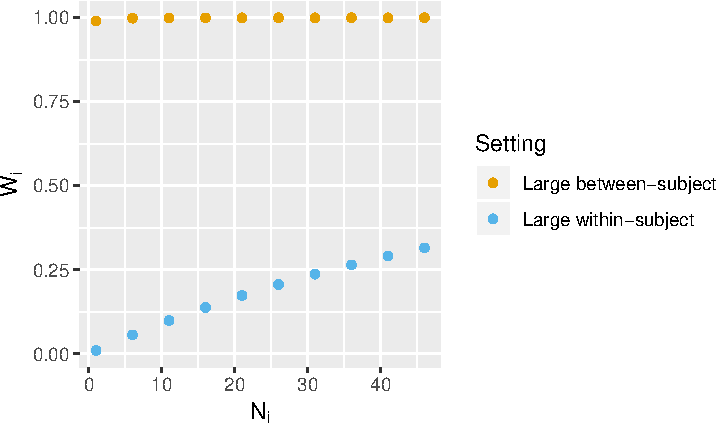
\includegraphics{3_video5_win_sub_mns_vs_cond_modes_files/figure-latex/unnamed-chunk-6-1} \end{center}

\hypertarget{summary-2}{%
\section{Summary}\label{summary-2}}

The settings in the above were pretty dramatic, but do show the 2SSS approach will likely be very similar to the mixed model result if the between-subject variance is large with respect to the size of the within-subject variance. Further, the weights will vary most across subjects if the sample sizes vary wildly. I would like to highly encourage the reader to run the above code with more settings to see how the weights change.

In the next chapter we will study the group results in more detail, but where the goal isn't a single group mean, but the difference in means between two groups. Does the 2SSS still work okay is most situations? What if one group has generally less data per subject than the other group? Can that cause false positives or reduced power in the mixed model result? What if we use the conditional modes in an analysis? Does that work okay? All of these questions will be addressed in the next chapter.

\hypertarget{v6-model-strategy-comparison---group-differences}{%
\chapter{V6: Model strategy comparison - group differences}\label{v6-model-strategy-comparison---group-differences}}

\hypertarget{group-differences-of-within-subject-averages-how-do-modeling-approaches-compare-with-unequal-groups-and-unequal-observations-within-subject}{%
\section{Group differences of within-subject averages: How do modeling approaches compare with unequal groups and unequal observations within-subject?}\label{group-differences-of-within-subject-averages-how-do-modeling-approaches-compare-with-unequal-groups-and-unequal-observations-within-subject}}

\hypertarget{introduction-4}{%
\section{Introduction}\label{introduction-4}}

This chapter accompanies the 6th video in the series, \href{https://youtu.be/C4r20a_pqlA}{``Can the regularization in mixed models be problematic?''}. Previous chapters focused on the regularization built into a mixed model. As I mentioned earlier, when I explained this to a colleague of mine, she asked how the regularization would impact her results. She's studying a patient group that tends to be much smaller than her control group and often she also has less data per subject in her patient group. Will the regularization of the mixed model hurt her power to detect group differences? In this chapter I focus on different approaches to modeling the data (mixed models, 2SSS and two pseudo 2SSS approaches) to investigate type I error and power when data are both balanced and unbalanced within-group and within-subject. Additionally, these simulations will address my previous comments about why the conditional modes are not the perfect way of viewing regularization.

\hypertarget{modeling-strategies-considered}{%
\subsection{Modeling strategies considered}\label{modeling-strategies-considered}}

There are four modeling approaches, total. First, the standard mixed model, with the group variable as a fixed effect and a random intercept. Second, the 2SSS using OLS at both stages. The last two models are similar to 2SSS, but for the first stage use conditional mode-based subject estimates from each of two different mixed models: one that models group as a fixed effect and one that does not. Although it is easy to argue that neither of these pseudo 2SSS models makes any sense, I can assure you that I have definitely seen this done in practice and therefore wanted to discuss it here. As we will see, neither of these approaches is a good idea. Surely, the second pseudo 2SSS model is most nonsensical since the model from which the conditional modes are extracted actually contains the inference of interest (group difference). Why do that extra work?

First think through how each of these approaches might behave. The 2SSS approach will not deal with the differing number of time points, so I would expect to see some issues there due to the variance differences between groups. For the mixed model there shouldn't be an issue. Sure, there could be some regularization, but since each group's mean is modeled, the bias would be toward the group means and not the overall mean. The conditional modes from the model with an intercept only will definitely yield some bias that could hide or emphasize the difference between groups. Also, the extra variability introduced by using these predicted values will likely lead to an underestimate of the variance. The 2SSS with conditional modes from the two group mixed model should have less bias, but the variance estimates will still be incorrect.

A very important consideration when you are interested in power, is you must first verify the type I error is controlled. That is how these simulations are set up. For the type I error investigation, the group means are set equal to each other. Then power is investigated in all scenarios, but it is very important to ignore the power estimates for the models that were not found to have controlled type I error. For that reason I have only put ``ghosts'' of the power estimates for those models in the plots. Bias is also important. Obviously the mixed model's conditional modes will be biased on purpose, but we don't want our final estimates to also be biased, because that can be misleading. You should suspect the pseudo 2SSS using conditional modes from the mixed model without modeling group will have a biased group difference estimate.

In the following the function for data simulation is constructed first, followed by a function that runs the analyses on numerous data sets so type I error and power can be calculated. After that I run 4 simulations for different study designs investigating type I error. Last power is estimated across the four designs. You are highly encouraged to try out your own designs. I have made the functions fairly flexible so you could do so. Do keep in mind that quite a few simulations are required and so it will take some time for them to complete.

\hypertarget{functions-for-data-simulation-and-analyses}{%
\section{Functions for data simulation and analyses}\label{functions-for-data-simulation-and-analyses}}

This first function simulates data for two groups. The code should seem very familiar, since it is based on the previous chapters that simulated data using the 2 stage approach. The one difference is there is a group variable here, while the previous simulations were for a single group.

\begin{Shaded}
\begin{Highlighting}[]
\KeywordTok{library}\NormalTok{(lme4)}
\KeywordTok{library}\NormalTok{(lmerTest)}
\KeywordTok{library}\NormalTok{(ggplot2)}
\KeywordTok{library}\NormalTok{(knitr)}
\KeywordTok{library}\NormalTok{(tidyverse)}
\KeywordTok{library}\NormalTok{(ggpubr)}

\NormalTok{make.data.grps =}\StringTok{ }\ControlFlowTok{function}\NormalTok{(win, btwn, n.win.sub, group.vec, grp1.mean, grp2.mean)\{}
  \CommentTok{\#win:  A vector of the within{-}subject sd of length nsub}
  \CommentTok{\#btwn: Scalar, the between{-}subject sd}
  \CommentTok{\# group.vec: 1\textquotesingle{}s and 0\textquotesingle{}s indicating group membership.  Length nsub.}
  \CommentTok{\# grp1.mean:  Mean for group 1 (group.vec=0)}
  \CommentTok{\# grp2.mean:  Mean for group 2 (group.vec=1)}
  
\NormalTok{  nsub =}\StringTok{ }\KeywordTok{length}\NormalTok{(group.vec)}
  \CommentTok{\# Simulate means for each subject}
\NormalTok{  mns.sub =}\StringTok{ }\NormalTok{grp1.mean}\OperatorTok{*}\NormalTok{group.vec }\OperatorTok{+}\StringTok{ }\NormalTok{(}\DecValTok{1}\OperatorTok{{-}}\NormalTok{group.vec)}\OperatorTok{*}\NormalTok{grp2.mean }\OperatorTok{+}\StringTok{  }\KeywordTok{rnorm}\NormalTok{(nsub, }\DataTypeTok{mean =} \DecValTok{0}\NormalTok{, }\DataTypeTok{sd =}\NormalTok{ btwn)}
  \CommentTok{\# Simulate data within{-}subject}
\NormalTok{  y =}\KeywordTok{c}\NormalTok{()}
\NormalTok{  id =}\StringTok{ }\KeywordTok{c}\NormalTok{()}
\NormalTok{  grp.all =}\StringTok{ }\KeywordTok{c}\NormalTok{()}
  \ControlFlowTok{for}\NormalTok{ (i }\ControlFlowTok{in} \DecValTok{1}\OperatorTok{:}\NormalTok{nsub)\{}
\NormalTok{    y.loop =}\StringTok{ }\KeywordTok{rnorm}\NormalTok{(n.win.sub[i], }
                   \DataTypeTok{mean =}\NormalTok{ mns.sub[i], }\DataTypeTok{sd =}\NormalTok{ win[i])}
\NormalTok{    y =}\StringTok{ }\KeywordTok{c}\NormalTok{(y, y.loop)}
\NormalTok{    id =}\StringTok{ }\KeywordTok{c}\NormalTok{(id, }\KeywordTok{rep}\NormalTok{(i, n.win.sub[i]))}
\NormalTok{   grp.all =}\StringTok{ }\KeywordTok{c}\NormalTok{(grp.all, }\KeywordTok{rep}\NormalTok{(group.vec[i], n.win.sub[i]))}
\NormalTok{  \}}
\NormalTok{  id =}\StringTok{ }\KeywordTok{as.factor}\NormalTok{(id)}
\NormalTok{  dat.mod =}\StringTok{ }\KeywordTok{data.frame}\NormalTok{(id, y, grp.all)}
  \KeywordTok{return}\NormalTok{(dat.mod)}
\NormalTok{\}}
\end{Highlighting}
\end{Shaded}

This function is created to run the simulation and organize the output. We will investigate the mean estimates for each group, the standard error of the difference in means according to each model, and the p-values, which will be used to either calculate power or type I error.

\begin{Shaded}
\begin{Highlighting}[]
\NormalTok{run.sim =}\StringTok{ }\ControlFlowTok{function}\NormalTok{(nsim, win, n.win.sub, btwn,  group.vec, grp1.mean, grp2.mean, rand.ord.nsub)\{}
  \CommentTok{\#nsim:  Number of simulations}
  \CommentTok{\#win: within{-}subject variances.  Vector of length nsub}
  \CommentTok{\#n.win.sub:  Number of measures within{-}subject.  Vector of length nsub}
  \CommentTok{\#btwn:  between{-}subject variance}
  \CommentTok{\#group.vec:  1/0 vector indicating groups}
  \CommentTok{\#grp1.mean, grp2.mean:  Group means}
  \CommentTok{\#rand.ord.nsub:  Randomly order subjects (mixes up n.win.sub so random subjects have smaller n)}
 
\NormalTok{  g1.mean.lmer =}\StringTok{ }\KeywordTok{rep}\NormalTok{(}\OtherTok{NA}\NormalTok{, nsim)}
\NormalTok{  g2.mean.lmer =}\StringTok{ }\KeywordTok{rep}\NormalTok{(}\OtherTok{NA}\NormalTok{, nsim)}
\NormalTok{  g1.mean}\FloatTok{.2}\NormalTok{sss =}\StringTok{ }\KeywordTok{rep}\NormalTok{(}\OtherTok{NA}\NormalTok{, nsim)}
\NormalTok{  g2.mean}\FloatTok{.2}\NormalTok{sss =}\StringTok{ }\KeywordTok{rep}\NormalTok{(}\OtherTok{NA}\NormalTok{, nsim)}
\NormalTok{  g1.mean}\FloatTok{.2}\NormalTok{sss.cond.mode}\FloatTok{.2}\NormalTok{grp =}\StringTok{ }\KeywordTok{rep}\NormalTok{(}\OtherTok{NA}\NormalTok{, nsim)}
\NormalTok{  g2.mean}\FloatTok{.2}\NormalTok{sss.cond.mode}\FloatTok{.2}\NormalTok{grp =}\StringTok{ }\KeywordTok{rep}\NormalTok{(}\OtherTok{NA}\NormalTok{, nsim)}
\NormalTok{  g1.mean}\FloatTok{.2}\NormalTok{sss.cond.mode.nogrp =}\StringTok{ }\KeywordTok{rep}\NormalTok{(}\OtherTok{NA}\NormalTok{, nsim)}
\NormalTok{  g2.mean}\FloatTok{.2}\NormalTok{sss.cond.mode.nogrp =}\StringTok{ }\KeywordTok{rep}\NormalTok{(}\OtherTok{NA}\NormalTok{, nsim)}
  
\NormalTok{  diff.se.lmer =}\StringTok{ }\KeywordTok{rep}\NormalTok{(}\OtherTok{NA}\NormalTok{, nsim)}
\NormalTok{  diff.se}\FloatTok{.2}\NormalTok{sss =}\StringTok{ }\KeywordTok{rep}\NormalTok{(}\OtherTok{NA}\NormalTok{, nsim)}
\NormalTok{  diff.se}\FloatTok{.2}\NormalTok{sss.cond.mode}\FloatTok{.2}\NormalTok{grp =}\StringTok{ }\KeywordTok{rep}\NormalTok{(}\OtherTok{NA}\NormalTok{, nsim)}
\NormalTok{  diff.se}\FloatTok{.2}\NormalTok{sss.cond.mode.nogrp =}\StringTok{ }\KeywordTok{rep}\NormalTok{(}\OtherTok{NA}\NormalTok{, nsim)}
  
\NormalTok{  p.lmer =}\StringTok{ }\KeywordTok{rep}\NormalTok{(}\OtherTok{NA}\NormalTok{, nsim)}
\NormalTok{  p}\FloatTok{.2}\NormalTok{sss =}\StringTok{ }\KeywordTok{rep}\NormalTok{(}\OtherTok{NA}\NormalTok{, nsim)}
\NormalTok{  p}\FloatTok{.2}\NormalTok{sss.cond.mode}\FloatTok{.2}\NormalTok{grp =}\StringTok{ }\KeywordTok{rep}\NormalTok{(}\OtherTok{NA}\NormalTok{, nsim)}
\NormalTok{  p}\FloatTok{.2}\NormalTok{sss.cond.mode.nogrp =}\StringTok{ }\KeywordTok{rep}\NormalTok{(}\OtherTok{NA}\NormalTok{, nsim)}
  
  \ControlFlowTok{for}\NormalTok{ (i }\ControlFlowTok{in} \DecValTok{1}\OperatorTok{:}\NormalTok{nsim) \{}
     \CommentTok{\# This is used when I want to randomly }
     \CommentTok{\#  select who has less data}
\NormalTok{    nsub =}\StringTok{ }\KeywordTok{length}\NormalTok{(group.vec)}
    \ControlFlowTok{if}\NormalTok{ (rand.ord.nsub }\OperatorTok{==}\StringTok{ \textquotesingle{}yes\textquotesingle{}}\NormalTok{)\{}
\NormalTok{      n.win.sub =}\StringTok{ }\KeywordTok{sample}\NormalTok{(n.win.sub)}
\NormalTok{    \}}
  
    \CommentTok{\# Generate the data}
\NormalTok{    dat.mod =}\StringTok{ }\KeywordTok{make.data.grps}\NormalTok{(win, btwn, n.win.sub,}
\NormalTok{                             group.vec, grp1.mean,}
\NormalTok{                             grp2.mean)}
  
    \CommentTok{\# Run the 4 models}
    \CommentTok{\# mixed model}
\NormalTok{    mod.lmer =}\StringTok{ }\KeywordTok{lmer}\NormalTok{(y }\OperatorTok{\textasciitilde{}}\StringTok{ }\DecValTok{1} \OperatorTok{+}\StringTok{ }\NormalTok{grp.all }\OperatorTok{+}\StringTok{ }\NormalTok{(}\DecValTok{1} \OperatorTok{|}\StringTok{ }\NormalTok{id), dat.mod)}

    \CommentTok{\# 2SSS OLS}
    \CommentTok{\# trick for getting OLS means for each subject}
\NormalTok{    ols.stage1 =}\StringTok{ }\KeywordTok{lm}\NormalTok{(y }\OperatorTok{\textasciitilde{}}\StringTok{ }\NormalTok{id }\DecValTok{{-}1}\NormalTok{, dat.mod)}\OperatorTok{$}\NormalTok{coeff}
\NormalTok{    twosss =}\StringTok{ }\KeywordTok{lm}\NormalTok{(ols.stage1 }\OperatorTok{\textasciitilde{}}\StringTok{ }\NormalTok{group.vec)}
    
    \CommentTok{\# 2SSS using cond modes from model including group}
    \CommentTok{\# pull out conditional modes}
\NormalTok{    cond.modes}\FloatTok{.2}\NormalTok{grp.mod =}\StringTok{ }\KeywordTok{coef}\NormalTok{(mod.lmer)}\OperatorTok{$}\NormalTok{id[, }\DecValTok{1}\NormalTok{]}\OperatorTok{+}
\StringTok{                          }\KeywordTok{coef}\NormalTok{(mod.lmer)}\OperatorTok{$}\NormalTok{id[, }\DecValTok{2}\NormalTok{]}\OperatorTok{*}\NormalTok{group.vec}
\NormalTok{    twosss.cond.mode}\FloatTok{.2}\NormalTok{grp =}\StringTok{ }\KeywordTok{lm}\NormalTok{(cond.modes}\FloatTok{.2}\NormalTok{grp.mod }\OperatorTok{\textasciitilde{}}
\StringTok{                                 }\NormalTok{group.vec)}
    \CommentTok{\#2SSS using cond modes from model without group  }
\NormalTok{    mod.lmer.nogroup =}\StringTok{ }\KeywordTok{lmer}\NormalTok{(y }\OperatorTok{\textasciitilde{}}\StringTok{ }\DecValTok{1} \OperatorTok{+}\StringTok{ }\NormalTok{(}\DecValTok{1} \OperatorTok{|}\StringTok{ }\NormalTok{id), dat.mod)}
\NormalTok{    cond.modes.nogroup.mod =}\StringTok{ }\KeywordTok{coef}\NormalTok{(mod.lmer.nogroup)}\OperatorTok{$}\NormalTok{id[, }\DecValTok{1}\NormalTok{]}
\NormalTok{    twosss.cond.mode.nogrp =}\StringTok{ }\KeywordTok{lm}\NormalTok{(cond.modes.nogroup.mod }\OperatorTok{\textasciitilde{}}
\StringTok{                                  }\NormalTok{group.vec)}
    
\NormalTok{    g1.mean.lmer[i] =}\StringTok{ }\KeywordTok{sum}\NormalTok{(}\KeywordTok{fixef}\NormalTok{(mod.lmer))}
\NormalTok{    g2.mean.lmer[i] =}\StringTok{ }\KeywordTok{fixef}\NormalTok{(mod.lmer)[}\DecValTok{1}\NormalTok{]}
\NormalTok{    g1.mean}\FloatTok{.2}\NormalTok{sss[i] =}\StringTok{ }\KeywordTok{sum}\NormalTok{(}\KeywordTok{coef}\NormalTok{(twosss))}
\NormalTok{    g2.mean}\FloatTok{.2}\NormalTok{sss[i] =}\StringTok{ }\KeywordTok{coef}\NormalTok{(twosss)[}\DecValTok{1}\NormalTok{]}
\NormalTok{    g1.mean}\FloatTok{.2}\NormalTok{sss.cond.mode}\FloatTok{.2}\NormalTok{grp[i] =}\StringTok{ }\KeywordTok{sum}\NormalTok{(}\KeywordTok{coef}\NormalTok{(twosss.cond.mode}\FloatTok{.2}\NormalTok{grp))}
\NormalTok{    g2.mean}\FloatTok{.2}\NormalTok{sss.cond.mode}\FloatTok{.2}\NormalTok{grp[i] =}\StringTok{ }\KeywordTok{coef}\NormalTok{(twosss.cond.mode}\FloatTok{.2}\NormalTok{grp)[}\DecValTok{1}\NormalTok{]}
\NormalTok{    g1.mean}\FloatTok{.2}\NormalTok{sss.cond.mode.nogrp[i] =}\StringTok{ }\KeywordTok{sum}\NormalTok{(}\KeywordTok{coef}\NormalTok{(twosss.cond.mode.nogrp))}
\NormalTok{    g2.mean}\FloatTok{.2}\NormalTok{sss.cond.mode.nogrp[i] =}\StringTok{ }\KeywordTok{coef}\NormalTok{(twosss.cond.mode.nogrp)[}\DecValTok{1}\NormalTok{]}
  
\NormalTok{    diff.se.lmer[i] =}\StringTok{ }\KeywordTok{summary}\NormalTok{(mod.lmer)}\OperatorTok{$}\NormalTok{coeff[}\DecValTok{2}\NormalTok{,}\DecValTok{2}\NormalTok{]}
\NormalTok{    diff.se}\FloatTok{.2}\NormalTok{sss[i] =}\StringTok{ }\KeywordTok{summary}\NormalTok{(twosss)}\OperatorTok{$}\NormalTok{coeff[}\DecValTok{2}\NormalTok{,}\DecValTok{2}\NormalTok{]}
\NormalTok{    diff.se}\FloatTok{.2}\NormalTok{sss.cond.mode}\FloatTok{.2}\NormalTok{grp[i] =}\StringTok{ }\KeywordTok{summary}\NormalTok{(twosss.cond.mode}\FloatTok{.2}\NormalTok{grp)}\OperatorTok{$}\NormalTok{coeff[}\DecValTok{2}\NormalTok{,}\DecValTok{2}\NormalTok{]}
\NormalTok{    diff.se}\FloatTok{.2}\NormalTok{sss.cond.mode.nogrp[i] =}\StringTok{ }\KeywordTok{summary}\NormalTok{(twosss.cond.mode.nogrp)}\OperatorTok{$}\NormalTok{coeff[}\DecValTok{2}\NormalTok{,}\DecValTok{2}\NormalTok{]}
  
\NormalTok{    p.lmer[i] =}\StringTok{ }\KeywordTok{summary}\NormalTok{(mod.lmer)}\OperatorTok{$}\NormalTok{coeff[}\DecValTok{2}\NormalTok{,}\DecValTok{5}\NormalTok{]}
\NormalTok{    p}\FloatTok{.2}\NormalTok{sss[i] =}\StringTok{ }\KeywordTok{summary}\NormalTok{(twosss)}\OperatorTok{$}\NormalTok{coeff[}\DecValTok{2}\NormalTok{,}\DecValTok{4}\NormalTok{]}
\NormalTok{    p}\FloatTok{.2}\NormalTok{sss.cond.mode}\FloatTok{.2}\NormalTok{grp[i] =}\StringTok{ }\KeywordTok{summary}\NormalTok{(twosss.cond.mode}\FloatTok{.2}\NormalTok{grp)}\OperatorTok{$}\NormalTok{coeff[}\DecValTok{2}\NormalTok{,}\DecValTok{4}\NormalTok{]}
\NormalTok{    p}\FloatTok{.2}\NormalTok{sss.cond.mode.nogrp[i] =}\StringTok{ }\KeywordTok{summary}\NormalTok{(twosss.cond.mode.nogrp)}\OperatorTok{$}\NormalTok{coeff[}\DecValTok{2}\NormalTok{,}\DecValTok{4}\NormalTok{]}
\NormalTok{  \}}
  
  \CommentTok{\# put it all into a data frame}
\NormalTok{  out =}\StringTok{ }\KeywordTok{data.frame}\NormalTok{(g1.mean.lmer, g2.mean.lmer, }
\NormalTok{                   g1.mean}\FloatTok{.2}\NormalTok{sss, g2.mean}\FloatTok{.2}\NormalTok{sss,}
\NormalTok{                   g1.mean}\FloatTok{.2}\NormalTok{sss.cond.mode}\FloatTok{.2}\NormalTok{grp,   }
\NormalTok{                   g2.mean}\FloatTok{.2}\NormalTok{sss.cond.mode}\FloatTok{.2}\NormalTok{grp,}
\NormalTok{                   g1.mean}\FloatTok{.2}\NormalTok{sss.cond.mode.nogrp,}
\NormalTok{                   g2.mean}\FloatTok{.2}\NormalTok{sss.cond.mode.nogrp,}
\NormalTok{                   diff.se.lmer, diff.se}\FloatTok{.2}\NormalTok{sss, diff.se}\FloatTok{.2}\NormalTok{sss.cond.mode}\FloatTok{.2}\NormalTok{grp, }
\NormalTok{                   diff.se}\FloatTok{.2}\NormalTok{sss.cond.mode.nogrp, p.lmer,}
\NormalTok{                   p}\FloatTok{.2}\NormalTok{sss, p}\FloatTok{.2}\NormalTok{sss.cond.mode}\FloatTok{.2}\NormalTok{grp,}
\NormalTok{                   p}\FloatTok{.2}\NormalTok{sss.cond.mode.nogrp)}
  \KeywordTok{return}\NormalTok{(out)}
\NormalTok{\}}
\end{Highlighting}
\end{Shaded}

\hypertarget{type-i-error}{%
\section{Type I error}\label{type-i-error}}

This first batch of simulations will calculate the type I error. In order to do so, the means for the groups are set to be equal (10). I would recommend at least 1000 simulations if you were to run this on your own. The code allows you to change the within-subject variance across subjects, but all model estimation methods assume a constant within-subject variance, so there wasn't really a reason to vary that here. Feel free to try it out on your own! I start of with balanced groups where either everybody has 30 observations or one group has 5 subjects with only 5 observations. Then, to mimic the real life data my colleague has where her patient group is much smaller and often have less data, I set the group sizes to 10 and 40 where they either all have 30 observations or half the patients only have 5 observations.

I realize the settings are a bit extreme, BUT if I can break a model in the extreme I will never ever use it on my real data. Why take the risk when I don't know how ``extreme'' my real data are. If I can't break a model in the extreme, then I know I can probably almost always trust that model.

By the way, if you've been paying close attention, take a look at the simulation settings and think back to the previous chapter. You will see there are differences in model performance here, but what would likely make them more similar? Hint: You'd need to change one number in the simulations I ran below. Again, aiming for the extreme to see what breaks!

\begin{Shaded}
\begin{Highlighting}[]
\CommentTok{\# 25 subjects each group, everybody has 30 observations}
\NormalTok{nsim =}\StringTok{ }\DecValTok{1000}
\NormalTok{win =}\StringTok{ }\KeywordTok{rep}\NormalTok{(}\DecValTok{10}\NormalTok{, }\DecValTok{50}\NormalTok{)}
\NormalTok{n.win.sub =}\StringTok{ }\KeywordTok{rep}\NormalTok{(}\DecValTok{30}\NormalTok{, }\DecValTok{50}\NormalTok{)}
\NormalTok{btwn =}\StringTok{ }\DecValTok{5}
\NormalTok{group.vec =}\StringTok{ }\KeywordTok{rep}\NormalTok{(}\KeywordTok{c}\NormalTok{(}\DecValTok{1}\NormalTok{, }\DecValTok{0}\NormalTok{), }\DataTypeTok{each =} \DecValTok{25}\NormalTok{)}
\CommentTok{\# Set the means equal, since we\textquotesingle{}re looking at Type I error}
\NormalTok{grp1.mean =}\StringTok{ }\DecValTok{10}
\NormalTok{grp2.mean =}\StringTok{ }\DecValTok{10}
\NormalTok{rand.ord.nsub =}\StringTok{ \textquotesingle{}no\textquotesingle{}}

\NormalTok{out.}\DecValTok{25}\NormalTok{.}\FloatTok{25.}\NormalTok{nolow.type1 =}\StringTok{ }\KeywordTok{run.sim}\NormalTok{(nsim, win, n.win.sub, btwn,}
\NormalTok{                          group.vec, grp1.mean, }
\NormalTok{                          grp2.mean, rand.ord.nsub)}

\CommentTok{\# Change so 5 in first group have low n}
\NormalTok{n.win.sub[}\DecValTok{1}\OperatorTok{:}\DecValTok{5}\NormalTok{] =}\StringTok{ }\DecValTok{5}
\NormalTok{out.}\DecValTok{25}\NormalTok{.}\FloatTok{25.5}\NormalTok{g1.type1 =}\StringTok{ }\KeywordTok{run.sim}\NormalTok{(nsim, win, n.win.sub, btwn,}
\NormalTok{                        group.vec, grp1.mean, }
\NormalTok{                        grp2.mean, rand.ord.nsub)}

\CommentTok{\#imblanaced groups with equal n}
\NormalTok{n.win.sub =}\StringTok{ }\KeywordTok{rep}\NormalTok{(}\DecValTok{30}\NormalTok{, }\DecValTok{50}\NormalTok{)}
\NormalTok{group.vec =}\StringTok{ }\KeywordTok{c}\NormalTok{(}\KeywordTok{rep}\NormalTok{(}\DecValTok{1}\NormalTok{, }\DecValTok{10}\NormalTok{), }\KeywordTok{rep}\NormalTok{(}\DecValTok{0}\NormalTok{, }\DecValTok{40}\NormalTok{))}
\NormalTok{out.}\DecValTok{10}\NormalTok{.}\FloatTok{40.}\NormalTok{nolow.type1 =}\StringTok{ }\KeywordTok{run.sim}\NormalTok{(nsim, win, n.win.sub, btwn,}
\NormalTok{                          group.vec, grp1.mean, grp2.mean,}
\NormalTok{                          rand.ord.nsub)}

\CommentTok{\# imbalanced groups with some in small group with low n}
\NormalTok{n.win.sub[}\DecValTok{1}\OperatorTok{:}\DecValTok{5}\NormalTok{] =}\StringTok{ }\DecValTok{5}
\NormalTok{out.}\DecValTok{10}\NormalTok{.}\FloatTok{40.5}\NormalTok{g1.type1 =}\StringTok{ }\KeywordTok{run.sim}\NormalTok{(nsim, win, n.win.sub, btwn, }
\NormalTok{                        group.vec, grp1.mean, grp2.mean,}
\NormalTok{                        rand.ord.nsub)}
\end{Highlighting}
\end{Shaded}

The following rearranges the data for plotting. First, the mean estimates (within each group and difference of means) are presented for each combination of data setup and analysis type. The boxplots are constructed from the estimates across the simulations. Look for bias in these estimates. Since the truth is known, I have overlayed lines to indicate the true value. Also, one would typically look to see if the estimates varied differently across the models. They do not in this case. There is a discussion about the plots after they are displayed.

\begin{Shaded}
\begin{Highlighting}[]
\CommentTok{\# arrange for plotting}

\NormalTok{cbPalette <{-}}\StringTok{ }\KeywordTok{c}\NormalTok{(}\StringTok{"\#E69F00"}\NormalTok{, }\StringTok{"\#56B4E9"}\NormalTok{, }\StringTok{"\#009E73"}\NormalTok{, }\StringTok{"\#F0E442"}\NormalTok{, }\StringTok{"\#0072B2"}\NormalTok{, }\StringTok{"\#D55E00"}\NormalTok{, }\StringTok{"\#CC79A7"}\NormalTok{,}\StringTok{"\#999999"}\NormalTok{)}

\NormalTok{ dat.all.type1 =}\StringTok{ }\KeywordTok{rbind}\NormalTok{(out.}\DecValTok{25}\NormalTok{.}\FloatTok{25.}\NormalTok{nolow.type1,}
\NormalTok{                       out.}\DecValTok{25}\NormalTok{.}\FloatTok{25.5}\NormalTok{g1.type1,}
\NormalTok{                       out.}\DecValTok{10}\NormalTok{.}\FloatTok{40.}\NormalTok{nolow.type1,}
\NormalTok{                       out.}\DecValTok{10}\NormalTok{.}\FloatTok{40.5}\NormalTok{g1.type1)}
 
\NormalTok{ dat.all.type1}\OperatorTok{$}\NormalTok{sim.type =}\StringTok{ }\KeywordTok{factor}\NormalTok{(}\KeywordTok{rep}\NormalTok{(}\KeywordTok{c}\NormalTok{(}\StringTok{"25.25.nolow"}\NormalTok{,}
                                       \StringTok{"25.25.5g1"}\NormalTok{,}
                                       \StringTok{"10.40.nolow"}\NormalTok{, }
                                       \StringTok{"10.40.5g1"}\NormalTok{),}
                                 \DataTypeTok{each =}\NormalTok{nsim), }\DataTypeTok{levels =}
                                 \KeywordTok{c}\NormalTok{(}\StringTok{"25.25.nolow"}\NormalTok{, }\StringTok{"25.25.5g1"}\NormalTok{,}
                                 \StringTok{"10.40.nolow"}\NormalTok{, }\StringTok{"10.40.5g1"}\NormalTok{))}
\NormalTok{ dat.all.type1}\OperatorTok{$}\NormalTok{n1 =}\StringTok{ }\KeywordTok{rep}\NormalTok{(}\KeywordTok{c}\NormalTok{(}\DecValTok{25}\NormalTok{, }\DecValTok{25}\NormalTok{, }\DecValTok{10}\NormalTok{, }\DecValTok{10}\NormalTok{), }\DataTypeTok{each =}\NormalTok{ nsim)}
\NormalTok{ dat.all.type1}\OperatorTok{$}\NormalTok{n2 =}\StringTok{ }\KeywordTok{rep}\NormalTok{(}\KeywordTok{c}\NormalTok{(}\DecValTok{25}\NormalTok{, }\DecValTok{25}\NormalTok{, }\DecValTok{40}\NormalTok{, }\DecValTok{40}\NormalTok{), }\DataTypeTok{each =}\NormalTok{ nsim)}
\NormalTok{ dat.all.type1}\OperatorTok{$}\NormalTok{lown =}\StringTok{ }\KeywordTok{rep}\NormalTok{(}\KeywordTok{c}\NormalTok{(}\StringTok{"none"}\NormalTok{, }\StringTok{"5 in g1"}\NormalTok{, }\StringTok{"none"}\NormalTok{, }
                            \StringTok{"5 in g1"}\NormalTok{),}
                          \DataTypeTok{each =}\NormalTok{ nsim)}
 
\NormalTok{ col.g1.mean =}\StringTok{ }\KeywordTok{grep}\NormalTok{(}\StringTok{\textquotesingle{}g1.mean\textquotesingle{}}\NormalTok{, }\KeywordTok{names}\NormalTok{(dat.all.type1), }
                    \DataTypeTok{fixed =}\NormalTok{ T)}
\NormalTok{ dat.all.g1.mean.type1 =}\StringTok{ }\NormalTok{dat.all.type1 }\OperatorTok{\%>\%}
\StringTok{                   }\KeywordTok{gather}\NormalTok{(}\DataTypeTok{key=}\StringTok{"key"}\NormalTok{, }
                          \DataTypeTok{value=}\StringTok{"group1mean"}\NormalTok{, }
\NormalTok{                          col.g1.mean) }\OperatorTok{\%>\%}
\StringTok{                   }\KeywordTok{separate}\NormalTok{(key, }
                            \KeywordTok{c}\NormalTok{(}\StringTok{"junk1"}\NormalTok{, }\StringTok{"model"}\NormalTok{), }
                            \DataTypeTok{sep =} \StringTok{"g1.mean."}\NormalTok{)}
\NormalTok{ dat.all.g1.mean.type1}\OperatorTok{$}\NormalTok{model =}\StringTok{ }\KeywordTok{factor}\NormalTok{(dat.all.g1.mean.type1}\OperatorTok{$}\NormalTok{model, }
                                \DataTypeTok{levels =} 
                                  \KeywordTok{c}\NormalTok{(}\StringTok{"lmer"}\NormalTok{, }\StringTok{"2sss"}\NormalTok{,}
                                   \StringTok{"2sss.cond.mode.nogrp"}\NormalTok{,}
                                    \StringTok{"2sss.cond.mode.2grp"}\NormalTok{))}
 
\NormalTok{g1.plot.type1 =}\StringTok{ }\KeywordTok{ggplot}\NormalTok{(dat.all.g1.mean.type1, }\KeywordTok{aes}\NormalTok{(}\DataTypeTok{x =}\NormalTok{ sim.type,}
                                      \DataTypeTok{y =}\NormalTok{ group1mean, }
                                      \DataTypeTok{fill =}\NormalTok{ model)) }\OperatorTok{+}
\StringTok{                }\KeywordTok{geom\_boxplot}\NormalTok{() }\OperatorTok{+}\StringTok{ }
\StringTok{                }\KeywordTok{geom\_hline}\NormalTok{(}\DataTypeTok{yintercept =} \DecValTok{10}\NormalTok{, }\DataTypeTok{color =} \StringTok{"gray26"}\NormalTok{) }\OperatorTok{+}
\StringTok{                }\KeywordTok{scale\_fill\_manual}\NormalTok{(}\DataTypeTok{values=}\NormalTok{cbPalette)}\OperatorTok{+}
\StringTok{                }\KeywordTok{ggtitle}\NormalTok{(}\StringTok{"Group 1 mean"}\NormalTok{)}

\CommentTok{\# Repeat for g2}
\NormalTok{col.g2.mean.type1 =}\StringTok{ }\KeywordTok{grep}\NormalTok{(}\StringTok{\textquotesingle{}g2.mean\textquotesingle{}}\NormalTok{, }\KeywordTok{names}\NormalTok{(dat.all.type1), }\DataTypeTok{fixed =}\NormalTok{ T)}
\NormalTok{dat.all.g2.mean.type1 =}\StringTok{ }\NormalTok{dat.all.type1 }\OperatorTok{\%>\%}
\StringTok{                   }\KeywordTok{gather}\NormalTok{(}\DataTypeTok{key=}\StringTok{"key"}\NormalTok{, }\DataTypeTok{value=}\StringTok{"group2mean"}\NormalTok{,}
\NormalTok{                          col.g2.mean.type1) }\OperatorTok{\%>\%}
\StringTok{                   }\KeywordTok{separate}\NormalTok{(key, }\KeywordTok{c}\NormalTok{(}\StringTok{"junk1"}\NormalTok{, }\StringTok{"model"}\NormalTok{), }
                            \DataTypeTok{sep =} \StringTok{"g2.mean."}\NormalTok{)}
\NormalTok{dat.all.g2.mean.type1}\OperatorTok{$}\NormalTok{model =}\StringTok{ }\KeywordTok{factor}\NormalTok{(dat.all.g2.mean.type1}\OperatorTok{$}\NormalTok{model, }
                                \DataTypeTok{levels =} \KeywordTok{c}\NormalTok{(}\StringTok{"lmer"}\NormalTok{, }\StringTok{"2sss"}\NormalTok{,}
                                      \StringTok{"2sss.cond.mode.nogrp"}\NormalTok{,}
                                      \StringTok{"2sss.cond.mode.2grp"}\NormalTok{)) }
\NormalTok{g2.plot.type1 =}\StringTok{ }\KeywordTok{ggplot}\NormalTok{(dat.all.g2.mean.type1, }
                       \KeywordTok{aes}\NormalTok{(}\DataTypeTok{x =}\NormalTok{ sim.type, }\DataTypeTok{y =}\NormalTok{ group2mean, }
                           \DataTypeTok{fill =}\NormalTok{ model)) }\OperatorTok{+}\StringTok{ }\KeywordTok{geom\_boxplot}\NormalTok{() }\OperatorTok{+}
\StringTok{                }\KeywordTok{geom\_hline}\NormalTok{(}\DataTypeTok{yintercept =} \DecValTok{10}\NormalTok{, }\DataTypeTok{color =} \StringTok{"gray26"}\NormalTok{)}\OperatorTok{+}
\StringTok{                }\KeywordTok{scale\_fill\_manual}\NormalTok{(}\DataTypeTok{values=}\NormalTok{cbPalette)}\OperatorTok{+}
\StringTok{                }\KeywordTok{ggtitle}\NormalTok{(}\StringTok{"Group 2 mean"}\NormalTok{)}
 
\CommentTok{\# Estimate the differences and then plot the differences}
\NormalTok{dat.all.diff.type1 =}\StringTok{ }\KeywordTok{left\_join}\NormalTok{(dat.all.g1.mean.type1, dat.all.g2.mean.type1)}
\NormalTok{dat.all.diff.type1}\OperatorTok{$}\NormalTok{diff =}\StringTok{ }\NormalTok{dat.all.diff.type1}\OperatorTok{$}\NormalTok{group2mean }\OperatorTok{{-}}
\StringTok{                    }\NormalTok{dat.all.diff.type1}\OperatorTok{$}\NormalTok{group1mean}
\NormalTok{dat.all.diff.type1}\OperatorTok{$}\NormalTok{model =}\StringTok{ }\KeywordTok{factor}\NormalTok{(dat.all.diff.type1}\OperatorTok{$}\NormalTok{model, }
                                \DataTypeTok{levels =} \KeywordTok{c}\NormalTok{(}\StringTok{"lmer"}\NormalTok{, }\StringTok{"2sss"}\NormalTok{,}
                                      \StringTok{"2sss.cond.mode.nogrp"}\NormalTok{,}
                                      \StringTok{"2sss.cond.mode.2grp"}\NormalTok{)) }
\NormalTok{diff.plot.type1 =}\StringTok{ }\KeywordTok{ggplot}\NormalTok{(dat.all.diff.type1, }\KeywordTok{aes}\NormalTok{(}\DataTypeTok{x =}\NormalTok{ sim.type, }
                                                 \DataTypeTok{y =}\NormalTok{ diff, }
                                                 \DataTypeTok{fill =}\NormalTok{ model)) }\OperatorTok{+}
\StringTok{                   }\KeywordTok{geom\_boxplot}\NormalTok{() }\OperatorTok{+}\StringTok{ }
\StringTok{                   }\KeywordTok{geom\_hline}\NormalTok{(}\DataTypeTok{yintercept =} \DecValTok{0}\NormalTok{, }\DataTypeTok{color =} \StringTok{"gray26"}\NormalTok{)}\OperatorTok{+}
\StringTok{                   }\KeywordTok{scale\_fill\_manual}\NormalTok{(}\DataTypeTok{values=}\NormalTok{cbPalette)}\OperatorTok{+}
\StringTok{                   }\KeywordTok{ggtitle}\NormalTok{(}\StringTok{"Difference"}\NormalTok{)}

\CommentTok{\# plot all 3 together}
\KeywordTok{ggarrange}\NormalTok{(g1.plot.type1, g2.plot.type1, diff.plot.type1, }\DataTypeTok{common.legend =} \OtherTok{TRUE}\NormalTok{,}
          \DataTypeTok{nrow =} \DecValTok{3}\NormalTok{, }\DataTypeTok{legend =} \StringTok{"right"}\NormalTok{)}
\end{Highlighting}
\end{Shaded}

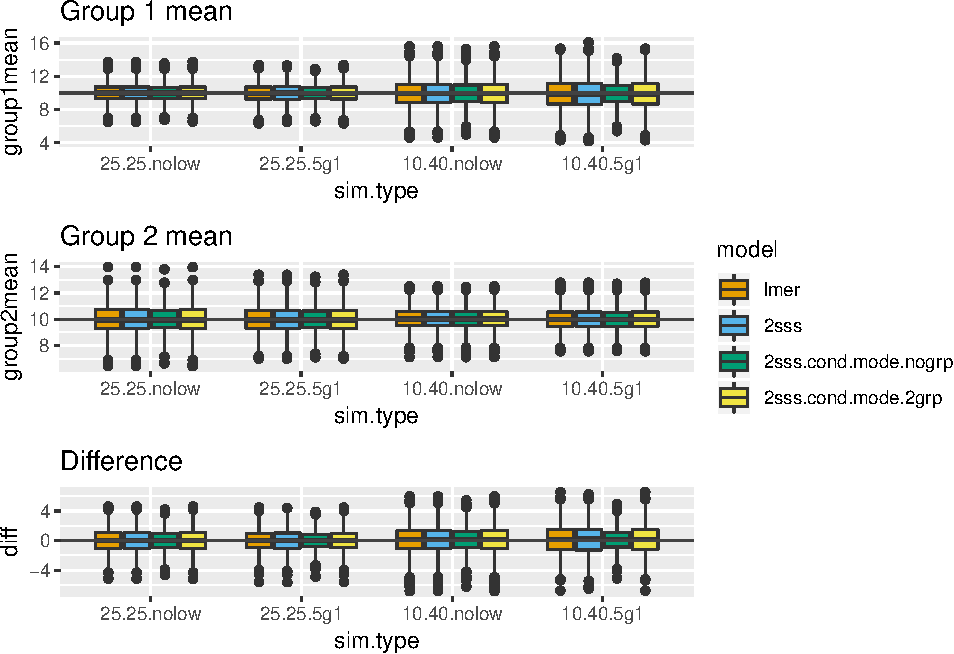
\includegraphics{4_video6_group_comparison_three_models_files/figure-latex/unnamed-chunk-4-1.pdf}

In the above plots, there is no bias present. This doesn't mean all methods are generally unbiased, it simply means when both group means are 0 there isn't bias. Think about how the regularization works in the mixed model and ask yourself whether it makes sense that there isn't bias here, even when some subjects have much less data. Do you predict there will be bias when the group means are different from each other?

Next the standard error of the group differences will be displayed. Generally we want our standard errors to be small BUT that's only helpful if our resulting inferences are valid (type I error is controlled). The setup is similar to the last plots.

\begin{Shaded}
\begin{Highlighting}[]
\CommentTok{\# Look at the standard errors}
\NormalTok{col.se.type1 =}\StringTok{ }\KeywordTok{grep}\NormalTok{(}\StringTok{\textquotesingle{}diff.se\textquotesingle{}}\NormalTok{, }\KeywordTok{names}\NormalTok{(dat.all.type1), }\DataTypeTok{fixed =}\NormalTok{ T)}
\NormalTok{dat.all.se.type1 =}\StringTok{ }\NormalTok{dat.all.type1 }\OperatorTok{\%>\%}
\StringTok{                   }\KeywordTok{gather}\NormalTok{(}\DataTypeTok{key=}\StringTok{"key"}\NormalTok{, }\DataTypeTok{value=}\StringTok{"se"}\NormalTok{, col.se.type1) }\OperatorTok{\%>\%}
\StringTok{                   }\KeywordTok{separate}\NormalTok{(key, }\KeywordTok{c}\NormalTok{(}\StringTok{"junk1"}\NormalTok{, }\StringTok{"model"}\NormalTok{), }
                            \DataTypeTok{sep =} \StringTok{"diff.se."}\NormalTok{)}
\NormalTok{dat.all.se.type1}\OperatorTok{$}\NormalTok{model =}\StringTok{ }\KeywordTok{factor}\NormalTok{(dat.all.se.type1}\OperatorTok{$}\NormalTok{model, }
                          \DataTypeTok{levels =} \KeywordTok{c}\NormalTok{(}\StringTok{"lmer"}\NormalTok{, }\StringTok{"2sss"}\NormalTok{,}
                                      \StringTok{"2sss.cond.mode.nogrp"}\NormalTok{,}
                                      \StringTok{"2sss.cond.mode.2grp"}\NormalTok{))}
 
\KeywordTok{ggplot}\NormalTok{(dat.all.se.type1, }\KeywordTok{aes}\NormalTok{(}\DataTypeTok{x =}\NormalTok{ sim.type, }\DataTypeTok{y =}\NormalTok{ se, }\DataTypeTok{fill =}\NormalTok{ model)) }\OperatorTok{+}
\StringTok{       }\KeywordTok{geom\_boxplot}\NormalTok{() }\OperatorTok{+}\StringTok{ }\KeywordTok{scale\_fill\_manual}\NormalTok{(}\DataTypeTok{values=}\NormalTok{cbPalette)}
\end{Highlighting}
\end{Shaded}

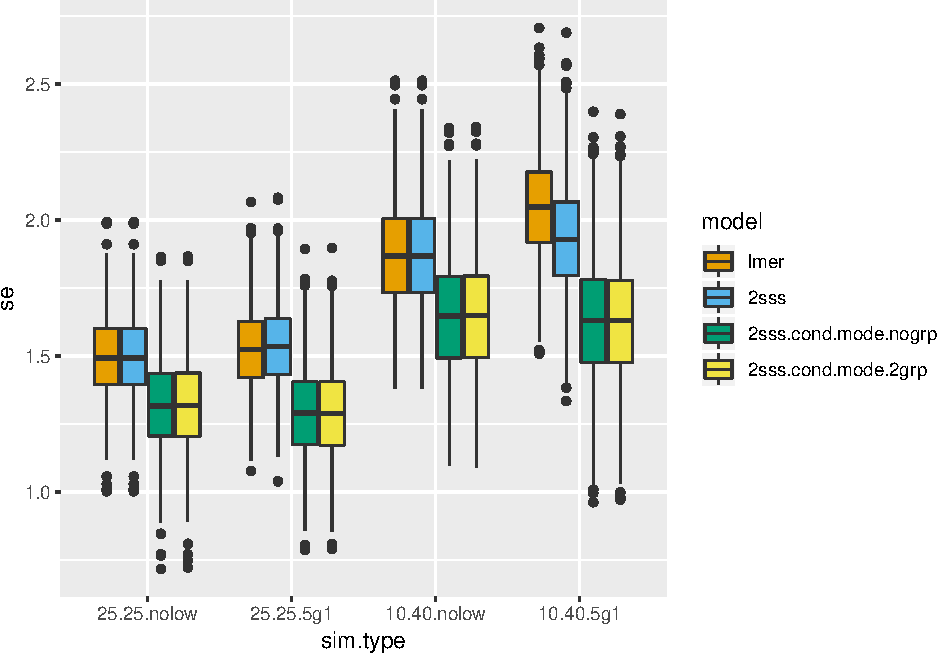
\includegraphics{4_video6_group_comparison_three_models_files/figure-latex/unnamed-chunk-5-1.pdf}

It is tempting to get excited about the pseudo 2SSS approaches that use conditional modes based on these standard error distributions BUT remember, we still haven't looked at type I error and fully investigated bias.

Next up is the type I error investigation, which clearly ends any hope one may have had for the 2SSS model using the conditional mode from the mixed model that had group included as a fixed effect. It doesn't matter in real life, though, since if one already ran that model they wouldn't have likely continued to extract conditional modes, etc, because the inference for the group difference was already included in the mixed model and, as the plot shows, the type I errors are preserved in those cases.

There are horizontal lines at 0.05 (solid) and the 95\% confidence interval (dashed). We will use type I error beyond the upper confidence bound as the threshold for an invalid test, which will be used to help interpret the power results later.

\begin{Shaded}
\begin{Highlighting}[]
 \CommentTok{\# Calculate type I error}
\NormalTok{ col.p =}\StringTok{ }\KeywordTok{grep}\NormalTok{(}\StringTok{\textquotesingle{}p.\textquotesingle{}}\NormalTok{, }\KeywordTok{names}\NormalTok{(dat.all.type1), }\DataTypeTok{fixed =}\NormalTok{ T)}
\NormalTok{ dat.all.p.type1 =}\StringTok{ }\NormalTok{dat.all.type1 }\OperatorTok{\%>\%}
\StringTok{              }\KeywordTok{gather}\NormalTok{(}\DataTypeTok{key=}\StringTok{"key"}\NormalTok{, }\DataTypeTok{value=}\StringTok{"pval"}\NormalTok{, col.p) }\OperatorTok{\%>\%}
\StringTok{              }\KeywordTok{separate}\NormalTok{(key, }\KeywordTok{c}\NormalTok{(}\StringTok{"junk1"}\NormalTok{, }\StringTok{"model"}\NormalTok{), }\DataTypeTok{sep =} \StringTok{"p."}\NormalTok{)}
\NormalTok{dat.all.p.type1}\OperatorTok{$}\NormalTok{p.sig =}\StringTok{ }\NormalTok{dat.all.p.type1}\OperatorTok{$}\NormalTok{pval }\OperatorTok{<=}\StringTok{ }\FloatTok{0.05}
\NormalTok{type1.mat =}\StringTok{ }\KeywordTok{aggregate}\NormalTok{(p.sig }\OperatorTok{\textasciitilde{}}\StringTok{ }\NormalTok{sim.type }\OperatorTok{+}\StringTok{ }\NormalTok{model,}
                    \DataTypeTok{data =}\NormalTok{ dat.all.p.type1, mean)}
\NormalTok{type1.mat}\OperatorTok{$}\NormalTok{model =}\StringTok{ }\KeywordTok{factor}\NormalTok{(type1.mat}\OperatorTok{$}\NormalTok{model, }
                       \DataTypeTok{levels =} \KeywordTok{c}\NormalTok{(}\StringTok{"lmer"}\NormalTok{, }\StringTok{"2sss"}\NormalTok{,}
                                  \StringTok{"2sss.cond.mode.nogrp"}\NormalTok{,}
                                  \StringTok{"2sss.cond.mode.2grp"}\NormalTok{))}

\CommentTok{\#bound for type I error (upper bound 95\% CI)}
\NormalTok{bound.up =}\StringTok{ }\FloatTok{.05}\OperatorTok{+}\KeywordTok{qnorm}\NormalTok{(}\DecValTok{1}\FloatTok{{-}0.05}\OperatorTok{/}\DecValTok{2}\NormalTok{)}\OperatorTok{*}\KeywordTok{sqrt}\NormalTok{(}\FloatTok{0.05}\OperatorTok{*}\NormalTok{(}\DecValTok{1}\FloatTok{{-}0.05}\NormalTok{)}\OperatorTok{/}\NormalTok{nsim)}
\NormalTok{bound.low =}\StringTok{ }\FloatTok{.05}\OperatorTok{{-}}\KeywordTok{qnorm}\NormalTok{(}\DecValTok{1}\FloatTok{{-}0.05}\OperatorTok{/}\DecValTok{2}\NormalTok{)}\OperatorTok{*}\KeywordTok{sqrt}\NormalTok{(}\FloatTok{0.05}\OperatorTok{*}\NormalTok{(}\DecValTok{1}\FloatTok{{-}0.05}\NormalTok{)}\OperatorTok{/}\NormalTok{nsim)}


\KeywordTok{ggplot}\NormalTok{(type1.mat, }\KeywordTok{aes}\NormalTok{(}\DataTypeTok{x=}\NormalTok{sim.type, }\DataTypeTok{y =}\NormalTok{ p.sig, }\DataTypeTok{fill =}\NormalTok{ model)) }\OperatorTok{+}\StringTok{ }\KeywordTok{geom\_bar}\NormalTok{(}\DataTypeTok{stat =} \StringTok{"identity"}\NormalTok{, }\DataTypeTok{position=}\KeywordTok{position\_dodge}\NormalTok{())}\OperatorTok{+}\StringTok{ }\KeywordTok{scale\_fill\_manual}\NormalTok{(}\DataTypeTok{values=}\NormalTok{cbPalette)}\OperatorTok{+}\StringTok{ }
\StringTok{  }\KeywordTok{geom\_hline}\NormalTok{(}\DataTypeTok{yintercept =}\NormalTok{ bound.up,}\DataTypeTok{color =} \StringTok{"gray26"}\NormalTok{, }\DataTypeTok{linetype =} \StringTok{"dashed"}\NormalTok{)}\OperatorTok{+}\StringTok{ }
\StringTok{  }\KeywordTok{geom\_hline}\NormalTok{(}\DataTypeTok{yintercept =}\NormalTok{ bound.low,}\DataTypeTok{color =} \StringTok{"gray26"}\NormalTok{, }\DataTypeTok{linetype =} \StringTok{"dashed"}\NormalTok{)}\OperatorTok{+}\StringTok{ }
\StringTok{  }\KeywordTok{geom\_hline}\NormalTok{(}\DataTypeTok{yintercept =} \FloatTok{0.05}\NormalTok{,}\DataTypeTok{color =} \StringTok{"gray26"}\NormalTok{)}
\end{Highlighting}
\end{Shaded}

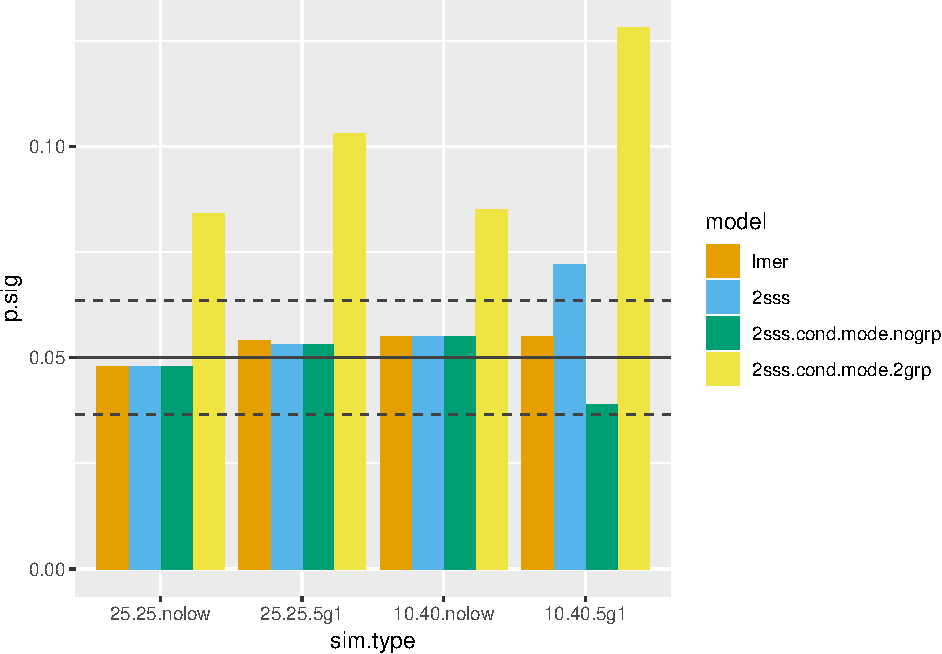
\includegraphics{4_video6_group_comparison_three_models_files/figure-latex/unnamed-chunk-6-1.pdf}

\begin{Shaded}
\begin{Highlighting}[]
\CommentTok{\# Add column that indicates when p is beyond upper bound}
\NormalTok{type1.mat}\OperatorTok{$}\NormalTok{valid =}\StringTok{ }\NormalTok{type1.mat}\OperatorTok{$}\NormalTok{p.sig}\OperatorTok{<}\NormalTok{bound.up}
\end{Highlighting}
\end{Shaded}

So far the 2SSS using conditional modes from the mixed model including group is a clear loser. Also, we can see that the OLS-based 2SSS fails when the smaller group has subjects with missing data. This actually makes complete sense since this is exactly what Welch's t-test is for! Specifically heteroscedasticity, which in this case is driven by the differing within-subject sample sizes. Standard OLS won't do anything for differing variances, but the mixed model does incorporate this information when the variance differences is driven by different sample sizes.

Last, the 2SSS approach where the conditional mode from the model without group looks somewhat hopeful here, but stay tuned. There's no avenue for bias to creep in due to the regularization here, since the means for both groups are set to zero!

\hypertarget{power}{%
\section{Power}\label{power}}

The same setup is used below, but the mean for the first group has been increased to 13, so the true difference between groups is 3. I haven't calculated what the true power should be in this case, so power will just be compared between different models within the same data type, but ignoring any power results for which the type I error was not controlled.

\begin{Shaded}
\begin{Highlighting}[]
\CommentTok{\# 25 subjects each group, everybody has 30 observations}
\NormalTok{win =}\StringTok{ }\KeywordTok{rep}\NormalTok{(}\DecValTok{10}\NormalTok{, }\DecValTok{50}\NormalTok{)}
\NormalTok{n.win.sub =}\StringTok{ }\KeywordTok{rep}\NormalTok{(}\DecValTok{30}\NormalTok{, }\DecValTok{50}\NormalTok{)}
\NormalTok{btwn =}\StringTok{ }\DecValTok{5}
\NormalTok{group.vec =}\StringTok{ }\KeywordTok{rep}\NormalTok{(}\KeywordTok{c}\NormalTok{(}\DecValTok{1}\NormalTok{, }\DecValTok{0}\NormalTok{), }\DataTypeTok{each =} \DecValTok{25}\NormalTok{)}
\NormalTok{grp1.mean =}\StringTok{ }\DecValTok{13}
\NormalTok{grp2.mean =}\StringTok{ }\DecValTok{10}
\NormalTok{rand.ord.nsub =}\StringTok{ \textquotesingle{}no\textquotesingle{}}

\NormalTok{out.}\DecValTok{25}\NormalTok{.}\FloatTok{25.}\NormalTok{nolow =}\StringTok{ }\KeywordTok{run.sim}\NormalTok{(nsim, win, n.win.sub, btwn,}
\NormalTok{                          group.vec, grp1.mean, }
\NormalTok{                          grp2.mean, rand.ord.nsub)}

\CommentTok{\# Change so 5 in first group have low n}
\NormalTok{n.win.sub[}\DecValTok{1}\OperatorTok{:}\DecValTok{5}\NormalTok{] =}\StringTok{ }\DecValTok{5}
\NormalTok{out.}\DecValTok{25}\NormalTok{.}\FloatTok{25.5}\NormalTok{g1 =}\StringTok{ }\KeywordTok{run.sim}\NormalTok{(nsim, win, n.win.sub, btwn,}
\NormalTok{                        group.vec, grp1.mean, }
\NormalTok{                        grp2.mean, rand.ord.nsub)}

\CommentTok{\#imblanaced groups with equal n}
\NormalTok{n.win.sub =}\StringTok{ }\KeywordTok{rep}\NormalTok{(}\DecValTok{30}\NormalTok{, }\DecValTok{50}\NormalTok{)}
\NormalTok{group.vec =}\StringTok{ }\KeywordTok{c}\NormalTok{(}\KeywordTok{rep}\NormalTok{(}\DecValTok{1}\NormalTok{, }\DecValTok{10}\NormalTok{), }\KeywordTok{rep}\NormalTok{(}\DecValTok{0}\NormalTok{, }\DecValTok{40}\NormalTok{))}
\NormalTok{out.}\DecValTok{10}\NormalTok{.}\FloatTok{40.}\NormalTok{nolow =}\StringTok{ }\KeywordTok{run.sim}\NormalTok{(nsim, win, n.win.sub, btwn,}
\NormalTok{                          group.vec, grp1.mean, grp2.mean,}
\NormalTok{                          rand.ord.nsub)}

\CommentTok{\# imbalanced groups with some in small group with low n}
\NormalTok{n.win.sub[}\DecValTok{1}\OperatorTok{:}\DecValTok{5}\NormalTok{] =}\StringTok{ }\DecValTok{5}
\NormalTok{out.}\DecValTok{10}\NormalTok{.}\FloatTok{40.5}\NormalTok{g1 =}\StringTok{ }\KeywordTok{run.sim}\NormalTok{(nsim, win, n.win.sub, btwn, }
\NormalTok{                        group.vec, grp1.mean, grp2.mean,}
\NormalTok{                        rand.ord.nsub)}
\end{Highlighting}
\end{Shaded}

Starting again with plots of the within-group means and mean difference. You can definitely see some bias showing. Try and understand where the bias is coming from and why it is in the direction it is. Even though all results are present here, recall we've written off the 2SSS using conditional modes from the mixed model that included group. Also, the 2SSS for imbalanced groups where one group has less data.

\begin{Shaded}
\begin{Highlighting}[]
\CommentTok{\# arrange for plotting}

\NormalTok{cbPalette <{-}}\StringTok{ }\KeywordTok{c}\NormalTok{(}\StringTok{"\#E69F00"}\NormalTok{, }\StringTok{"\#56B4E9"}\NormalTok{, }\StringTok{"\#009E73"}\NormalTok{, }\StringTok{"\#F0E442"}\NormalTok{, }\StringTok{"\#0072B2"}\NormalTok{, }\StringTok{"\#D55E00"}\NormalTok{, }\StringTok{"\#CC79A7"}\NormalTok{,}\StringTok{"\#999999"}\NormalTok{)}

\NormalTok{ dat.all =}\StringTok{ }\KeywordTok{rbind}\NormalTok{(out.}\DecValTok{25}\NormalTok{.}\FloatTok{25.}\NormalTok{nolow, out.}\DecValTok{25}\NormalTok{.}\FloatTok{25.5}\NormalTok{g1,}
\NormalTok{                 out.}\DecValTok{10}\NormalTok{.}\FloatTok{40.}\NormalTok{nolow, out.}\DecValTok{10}\NormalTok{.}\FloatTok{40.5}\NormalTok{g1)}
 
\NormalTok{ dat.all}\OperatorTok{$}\NormalTok{sim.type =}\StringTok{ }\KeywordTok{factor}\NormalTok{(}\KeywordTok{rep}\NormalTok{(}\KeywordTok{c}\NormalTok{(}\StringTok{"25.25.nolow"}\NormalTok{, }\StringTok{"25.25.5g1"}\NormalTok{,}
                                 \StringTok{"10.40.nolow"}\NormalTok{, }\StringTok{"10.40.5g1"}\NormalTok{),}
                               \DataTypeTok{each =}\NormalTok{nsim), }\DataTypeTok{levels =}
                             \KeywordTok{c}\NormalTok{(}\StringTok{"25.25.nolow"}\NormalTok{, }\StringTok{"25.25.5g1"}\NormalTok{,}
                               \StringTok{"10.40.nolow"}\NormalTok{, }\StringTok{"10.40.5g1"}\NormalTok{))}
\NormalTok{ dat.all}\OperatorTok{$}\NormalTok{n1 =}\StringTok{ }\KeywordTok{rep}\NormalTok{(}\KeywordTok{c}\NormalTok{(}\DecValTok{25}\NormalTok{, }\DecValTok{25}\NormalTok{, }\DecValTok{10}\NormalTok{, }\DecValTok{10}\NormalTok{), }\DataTypeTok{each =}\NormalTok{ nsim)}
\NormalTok{ dat.all}\OperatorTok{$}\NormalTok{n2 =}\StringTok{ }\KeywordTok{rep}\NormalTok{(}\KeywordTok{c}\NormalTok{(}\DecValTok{25}\NormalTok{, }\DecValTok{25}\NormalTok{, }\DecValTok{40}\NormalTok{, }\DecValTok{40}\NormalTok{), }\DataTypeTok{each =}\NormalTok{ nsim)}
\NormalTok{ dat.all}\OperatorTok{$}\NormalTok{lown =}\StringTok{ }\KeywordTok{rep}\NormalTok{(}\KeywordTok{c}\NormalTok{(}\StringTok{"none"}\NormalTok{, }\StringTok{"5 in g1"}\NormalTok{, }\StringTok{"none"}\NormalTok{, }\StringTok{"5 in g1"}\NormalTok{),}
                    \DataTypeTok{each =}\NormalTok{ nsim)}
 
 
\NormalTok{ col.g1.mean =}\StringTok{ }\KeywordTok{grep}\NormalTok{(}\StringTok{\textquotesingle{}g1.mean\textquotesingle{}}\NormalTok{, }\KeywordTok{names}\NormalTok{(dat.all), }\DataTypeTok{fixed =}\NormalTok{ T)}
\NormalTok{ dat.all.g1.mean =}\StringTok{ }\NormalTok{dat.all }\OperatorTok{\%>\%}
\StringTok{                   }\KeywordTok{gather}\NormalTok{(}\DataTypeTok{key=}\StringTok{"key"}\NormalTok{, }
                          \DataTypeTok{value=}\StringTok{"group1mean"}\NormalTok{, }
\NormalTok{                          col.g1.mean) }\OperatorTok{\%>\%}
\StringTok{                   }\KeywordTok{separate}\NormalTok{(key, }
                            \KeywordTok{c}\NormalTok{(}\StringTok{"junk1"}\NormalTok{, }\StringTok{"model"}\NormalTok{), }
                            \DataTypeTok{sep =} \StringTok{"g1.mean."}\NormalTok{)}
\NormalTok{ dat.all.g1.mean}\OperatorTok{$}\NormalTok{model =}\StringTok{ }\KeywordTok{factor}\NormalTok{(dat.all.g1.mean}\OperatorTok{$}\NormalTok{model, }
                                \DataTypeTok{levels =} 
                                  \KeywordTok{c}\NormalTok{(}\StringTok{"lmer"}\NormalTok{, }\StringTok{"2sss"}\NormalTok{,}
                                   \StringTok{"2sss.cond.mode.nogrp"}\NormalTok{,}
                                    \StringTok{"2sss.cond.mode.2grp"}\NormalTok{))}
 
\NormalTok{g1.plot =}\StringTok{ }\KeywordTok{ggplot}\NormalTok{(dat.all.g1.mean, }\KeywordTok{aes}\NormalTok{(}\DataTypeTok{x =}\NormalTok{ sim.type,}
                                      \DataTypeTok{y =}\NormalTok{ group1mean, }
                                      \DataTypeTok{fill =}\NormalTok{ model)) }\OperatorTok{+}
\StringTok{          }\KeywordTok{geom\_boxplot}\NormalTok{() }\OperatorTok{+}\StringTok{ }
\StringTok{          }\KeywordTok{geom\_hline}\NormalTok{(}\DataTypeTok{yintercept =} \DecValTok{13}\NormalTok{, }
                     \DataTypeTok{color =} \StringTok{"gray26"}\NormalTok{) }\OperatorTok{+}
\StringTok{          }\KeywordTok{scale\_fill\_manual}\NormalTok{(}\DataTypeTok{values=}\NormalTok{cbPalette)}\OperatorTok{+}
\StringTok{          }\KeywordTok{ggtitle}\NormalTok{(}\StringTok{"Group 1 mean"}\NormalTok{)}

\CommentTok{\# Repeat for g2}
\NormalTok{col.g2.mean =}\StringTok{ }\KeywordTok{grep}\NormalTok{(}\StringTok{\textquotesingle{}g2.mean\textquotesingle{}}\NormalTok{, }\KeywordTok{names}\NormalTok{(dat.all), }\DataTypeTok{fixed =}\NormalTok{ T)}
\NormalTok{dat.all.g2.mean =}\StringTok{ }\NormalTok{dat.all }\OperatorTok{\%>\%}
\StringTok{                   }\KeywordTok{gather}\NormalTok{(}\DataTypeTok{key=}\StringTok{"key"}\NormalTok{, }\DataTypeTok{value=}\StringTok{"group2mean"}\NormalTok{,}
\NormalTok{                          col.g2.mean) }\OperatorTok{\%>\%}
\StringTok{                   }\KeywordTok{separate}\NormalTok{(key, }\KeywordTok{c}\NormalTok{(}\StringTok{"junk1"}\NormalTok{, }\StringTok{"model"}\NormalTok{), }
                            \DataTypeTok{sep =} \StringTok{"g2.mean."}\NormalTok{)}
\NormalTok{dat.all.g2.mean}\OperatorTok{$}\NormalTok{model =}\StringTok{ }\KeywordTok{factor}\NormalTok{(dat.all.g2.mean}\OperatorTok{$}\NormalTok{model, }
                                \DataTypeTok{levels =} \KeywordTok{c}\NormalTok{(}\StringTok{"lmer"}\NormalTok{, }\StringTok{"2sss"}\NormalTok{,}
                                      \StringTok{"2sss.cond.mode.nogrp"}\NormalTok{,}
                                      \StringTok{"2sss.cond.mode.2grp"}\NormalTok{)) }
\NormalTok{g2.plot =}\StringTok{ }\KeywordTok{ggplot}\NormalTok{(dat.all.g2.mean, }\KeywordTok{aes}\NormalTok{(}\DataTypeTok{x =}\NormalTok{ sim.type, }\DataTypeTok{y =}\NormalTok{ group2mean, }\DataTypeTok{fill =}\NormalTok{ model)) }\OperatorTok{+}\StringTok{ }
\StringTok{        }\KeywordTok{geom\_boxplot}\NormalTok{() }\OperatorTok{+}\StringTok{ }
\StringTok{        }\KeywordTok{geom\_hline}\NormalTok{(}\DataTypeTok{yintercept =} \DecValTok{10}\NormalTok{, }\DataTypeTok{color =} \StringTok{"gray26"}\NormalTok{) }\OperatorTok{+}\StringTok{      }
\StringTok{        }\KeywordTok{scale\_fill\_manual}\NormalTok{(}\DataTypeTok{values=}\NormalTok{cbPalette)}\OperatorTok{+}\KeywordTok{ggtitle}\NormalTok{(}\StringTok{"Group 2 mean"}\NormalTok{)}
 
\CommentTok{\# Estimate the differences and then plot the differences}
\NormalTok{dat.all.diff =}\StringTok{ }\KeywordTok{left\_join}\NormalTok{(dat.all.g1.mean, dat.all.g2.mean)}
\NormalTok{dat.all.diff}\OperatorTok{$}\NormalTok{diff =}\StringTok{ }\NormalTok{dat.all.diff}\OperatorTok{$}\NormalTok{group2mean }\OperatorTok{{-}}
\StringTok{                    }\NormalTok{dat.all.diff}\OperatorTok{$}\NormalTok{group1mean}
\NormalTok{dat.all.diff}\OperatorTok{$}\NormalTok{model =}\StringTok{ }\KeywordTok{factor}\NormalTok{(dat.all.diff}\OperatorTok{$}\NormalTok{model, }
                                \DataTypeTok{levels =} \KeywordTok{c}\NormalTok{(}\StringTok{"lmer"}\NormalTok{, }\StringTok{"2sss"}\NormalTok{,}
                                      \StringTok{"2sss.cond.mode.nogrp"}\NormalTok{,}
                                      \StringTok{"2sss.cond.mode.2grp"}\NormalTok{)) }
\NormalTok{diff.plot =}\StringTok{ }\KeywordTok{ggplot}\NormalTok{(dat.all.diff, }\KeywordTok{aes}\NormalTok{(}\DataTypeTok{x =}\NormalTok{ sim.type, }\DataTypeTok{y =}\NormalTok{ diff,}
                                     \DataTypeTok{fill =}\NormalTok{ model)) }\OperatorTok{+}
\StringTok{            }\KeywordTok{geom\_boxplot}\NormalTok{() }\OperatorTok{+}\StringTok{ }\KeywordTok{geom\_hline}\NormalTok{(}\DataTypeTok{yintercept =} \DecValTok{{-}3}\NormalTok{,}
                                        \DataTypeTok{color =} \StringTok{"gray26"}\NormalTok{)}\OperatorTok{+}
\StringTok{            }\KeywordTok{scale\_fill\_manual}\NormalTok{(}\DataTypeTok{values=}\NormalTok{cbPalette)}\OperatorTok{+}
\StringTok{            }\KeywordTok{ggtitle}\NormalTok{(}\StringTok{"Difference"}\NormalTok{)}

\CommentTok{\# plot all 3 together}
\KeywordTok{ggarrange}\NormalTok{(g1.plot, g2.plot, diff.plot, }\DataTypeTok{common.legend =} \OtherTok{TRUE}\NormalTok{,}
          \DataTypeTok{nrow =} \DecValTok{3}\NormalTok{, }\DataTypeTok{legend =} \StringTok{"right"}\NormalTok{)}
\end{Highlighting}
\end{Shaded}

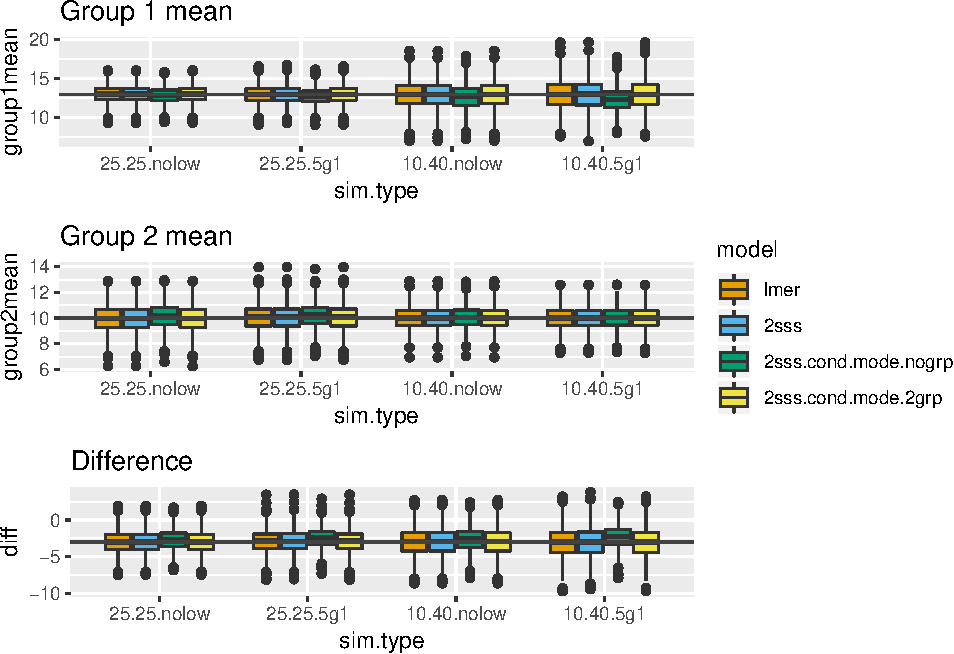
\includegraphics{4_video6_group_comparison_three_models_files/figure-latex/unnamed-chunk-8-1.pdf}

There is always some bias on the 2SSS approach that used conditional modes from the mixed model without a fixed effect for group. It gets worse when group 1 is small and some of those subjects only had 5 observations, because that's when the regularization will be strongest and the regularization is pulling the estimates toward the overall mean, not the mean of group 1. The bias is not present in the 2SSS model that uses the conditional modes from the mixed model with group because the bias in that case will be toward the group mean instead of the overall mean.

An important point to make here is the bias is in the direction of the null. So, although the standard errors are too small, this is overridden by the bias causing the difference estimate to also be too small.

Moving on to the standard errors, the results are similar to before.

\begin{Shaded}
\begin{Highlighting}[]
\CommentTok{\# Look at the standard errors}
\NormalTok{col.se =}\StringTok{ }\KeywordTok{grep}\NormalTok{(}\StringTok{\textquotesingle{}diff.se\textquotesingle{}}\NormalTok{, }\KeywordTok{names}\NormalTok{(dat.all), }\DataTypeTok{fixed =}\NormalTok{ T)}
\NormalTok{dat.all.se =}\StringTok{ }\NormalTok{dat.all }\OperatorTok{\%>\%}
\StringTok{                   }\KeywordTok{gather}\NormalTok{(}\DataTypeTok{key=}\StringTok{"key"}\NormalTok{, }\DataTypeTok{value=}\StringTok{"se"}\NormalTok{, col.se) }\OperatorTok{\%>\%}
\StringTok{                   }\KeywordTok{separate}\NormalTok{(key, }\KeywordTok{c}\NormalTok{(}\StringTok{"junk1"}\NormalTok{, }\StringTok{"model"}\NormalTok{), }
                            \DataTypeTok{sep =} \StringTok{"diff.se."}\NormalTok{)}
\NormalTok{ dat.all.se}\OperatorTok{$}\NormalTok{model =}\StringTok{ }\KeywordTok{factor}\NormalTok{(dat.all.se}\OperatorTok{$}\NormalTok{model, }
                          \DataTypeTok{levels =} \KeywordTok{c}\NormalTok{(}\StringTok{"lmer"}\NormalTok{, }\StringTok{"2sss"}\NormalTok{,}
                                      \StringTok{"2sss.cond.mode.nogrp"}\NormalTok{,}
                                      \StringTok{"2sss.cond.mode.2grp"}\NormalTok{))}
 
 \KeywordTok{ggplot}\NormalTok{(dat.all.se, }\KeywordTok{aes}\NormalTok{(}\DataTypeTok{x =}\NormalTok{ sim.type, }\DataTypeTok{y =}\NormalTok{ se, }\DataTypeTok{fill =}\NormalTok{ model)) }\OperatorTok{+}\StringTok{ }\KeywordTok{geom\_boxplot}\NormalTok{() }\OperatorTok{+}\StringTok{ }\KeywordTok{scale\_fill\_manual}\NormalTok{(}\DataTypeTok{values=}\NormalTok{cbPalette)}
\end{Highlighting}
\end{Shaded}

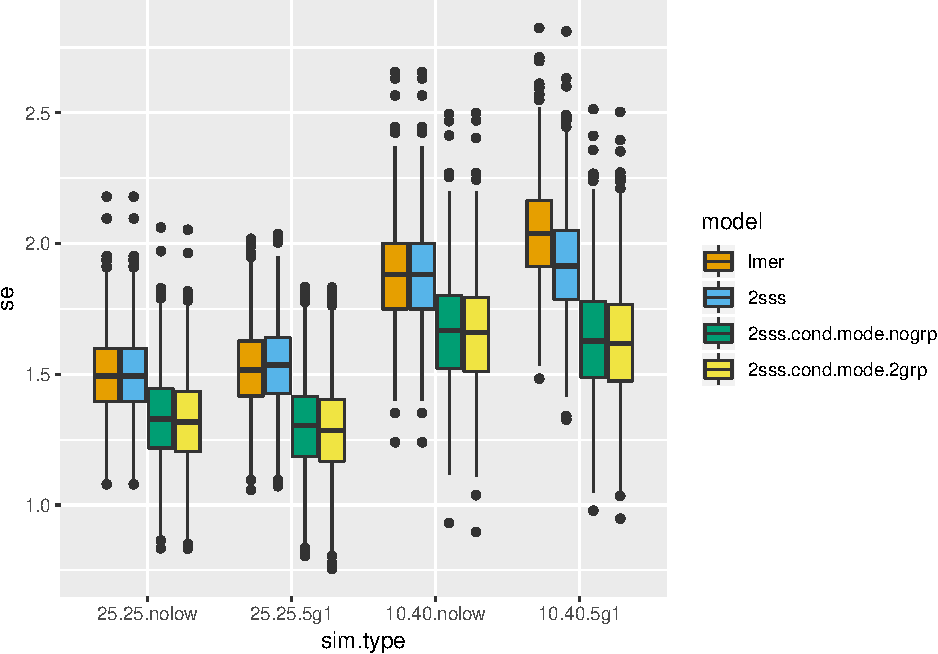
\includegraphics{4_video6_group_comparison_three_models_files/figure-latex/unnamed-chunk-9-1.pdf}

Last, but not least, power. I have faded out the bars of the power for the methods that were found to not be valid when type I error was estimated above.

\begin{Shaded}
\begin{Highlighting}[]
 \CommentTok{\# Calculate power}
\NormalTok{ col.p =}\StringTok{ }\KeywordTok{grep}\NormalTok{(}\StringTok{\textquotesingle{}p.\textquotesingle{}}\NormalTok{, }\KeywordTok{names}\NormalTok{(dat.all), }\DataTypeTok{fixed =}\NormalTok{ T)}
\NormalTok{ dat.all.p =}\StringTok{ }\NormalTok{dat.all }\OperatorTok{\%>\%}
\StringTok{              }\KeywordTok{gather}\NormalTok{(}\DataTypeTok{key=}\StringTok{"key"}\NormalTok{, }\DataTypeTok{value=}\StringTok{"pval"}\NormalTok{, col.p) }\OperatorTok{\%>\%}
\StringTok{              }\KeywordTok{separate}\NormalTok{(key, }\KeywordTok{c}\NormalTok{(}\StringTok{"junk1"}\NormalTok{, }\StringTok{"model"}\NormalTok{), }\DataTypeTok{sep =} \StringTok{"p."}\NormalTok{)}
\NormalTok{ dat.all.p}\OperatorTok{$}\NormalTok{p.sig =}\StringTok{ }\NormalTok{dat.all.p}\OperatorTok{$}\NormalTok{pval }\OperatorTok{<=}\StringTok{ }\FloatTok{0.05}
\NormalTok{pow.mat =}\StringTok{ }\KeywordTok{aggregate}\NormalTok{(p.sig }\OperatorTok{\textasciitilde{}}\StringTok{ }\NormalTok{sim.type }\OperatorTok{+}\StringTok{ }\NormalTok{model,}
                    \DataTypeTok{data =}\NormalTok{ dat.all.p, mean)}
\NormalTok{pow.mat}\OperatorTok{$}\NormalTok{model =}\StringTok{ }\KeywordTok{factor}\NormalTok{(pow.mat}\OperatorTok{$}\NormalTok{model, }
                       \DataTypeTok{levels =} \KeywordTok{c}\NormalTok{(}\StringTok{"lmer"}\NormalTok{, }\StringTok{"2sss"}\NormalTok{,}
                                  \StringTok{"2sss.cond.mode.nogrp"}\NormalTok{,}
                                  \StringTok{"2sss.cond.mode.2grp"}\NormalTok{))}
\CommentTok{\# Add in valid test info from type 1 error}
\NormalTok{valid.info =}\StringTok{ }\NormalTok{type1.mat[,}\KeywordTok{c}\NormalTok{(}\StringTok{"sim.type"}\NormalTok{, }\StringTok{"model"}\NormalTok{, }\StringTok{"valid"}\NormalTok{)]}
\NormalTok{pow.mat =}\StringTok{ }\KeywordTok{full\_join}\NormalTok{(pow.mat, valid.info)}

\KeywordTok{ggplot}\NormalTok{(pow.mat, }\KeywordTok{aes}\NormalTok{(}\DataTypeTok{x=}\NormalTok{sim.type, }\DataTypeTok{y =}\NormalTok{ p.sig, }\DataTypeTok{fill =}\NormalTok{ model, }\DataTypeTok{alpha =}\NormalTok{ valid)) }\OperatorTok{+}\StringTok{ }\KeywordTok{geom\_bar}\NormalTok{(}\DataTypeTok{stat =} \StringTok{"identity"}\NormalTok{, }\DataTypeTok{position=}\KeywordTok{position\_dodge}\NormalTok{())}\OperatorTok{+}\StringTok{ }\KeywordTok{scale\_fill\_manual}\NormalTok{(}\DataTypeTok{values=}\NormalTok{cbPalette)}\OperatorTok{+}\KeywordTok{scale\_alpha\_discrete}\NormalTok{(}\DataTypeTok{range =} \KeywordTok{c}\NormalTok{(}\FloatTok{0.2}\NormalTok{, }\DecValTok{1}\NormalTok{))}
\end{Highlighting}
\end{Shaded}

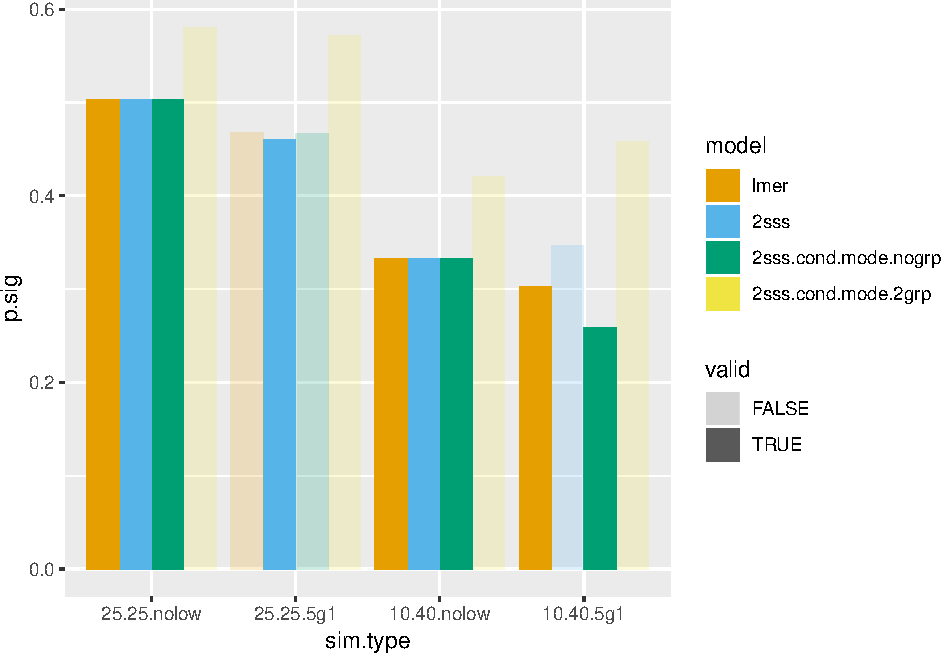
\includegraphics{4_video6_group_comparison_three_models_files/figure-latex/unnamed-chunk-10-1.pdf}

Firstly, the star of the show, not surprisingly, is lmer. Not only was type I error always, preserved, but it either ties for highest power or has the highest power. Also, remember it was only 1 simple line of code. The 2SSS almost looks like the winner when the patient group is smaller and some patients have fewer data points, but that test had inflated type I error, so the power cannot be considered. As far as the 2SSS approach using conditional modes from the mixed model without group, it seems like maybe this one is okay but remember that bias! Biased estimates aren't going to be of much use, so that model cannot be recommended.

\hypertarget{summary-3}{%
\section{Summary}\label{summary-3}}

Overall, when comparing group means the mixed model is the safest bet. The clear loser is the pseudo 2SSS using conditional modes from the model with group as a fixed effect. The OLS-based 2SSS approach might be okay in a pinch if your groups are balanced and data within-subject are balanced, but I will remind you the mixed model was a single line of code. The psuedo 2SSS approach with conditional modes extracted from the mixed model without an intercept may yield biased results, due to the regularization, so it should also be avoided.

I would like to circle back to when I used the conditional modes to illustrate the regularization earlier. I kept mentioning that they were not perfect and these simulations show why. The estimates from the 2SSS approach using conditional modes that modeled group were extracted from the exact same model used for the lmer results, yet look how different the performance is! I know it is often the case that these values are plotted in manuscripts to help understand what the individual subjects were doing BUT it is very important when you make plots that they are representative of what the model was actually doing. In this case it can be misleading so I would recommend one be careful if using such plots and make sure the reader understands that the values are simply predictions with high variability and do not perfectly represent how individual subjects behaved in the model. Again, this is because the mixed model isn't actually using those estimates and those estimates are very noisy predictions. So, they were nice for visualizing how the regularization works, but they are not the same as what is going on inside of the model!

If you haven't already figured it out, I have set the between-subject variance to be quite small here. If increased, the results will be more similar across modeling approaches. Since we don't know what our true within- and between-subject variances are, I would never assume the between subject was large enough that I didn't need to worry when it is often the case that I can simply use the appropriate model.

\end{document}
